
%% CLASS MANUAL FOUND IN http://blog.poormansmath.net/latex-class-for-lecture-notes/ %%
%% CLASS AUTHOR Stefano Maggiolo %%


\documentclass[english,course,draft]{Notes}
\title{ INTRODUCTORY ECONOMICS}
\subject{Economics}
\author{Joao Almeida-Domingues}
\email{2334590D@student.gla.ac.uk}
\speaker{Dr. Constantine Sorokin}
\date{07}{01}{2019}
\dateend{24}{05}{2019}
\place{University of Glasgow}


\usepackage[backend=biber, style=reading]{biblatex}
\bibliography{refEco}
\usepackage{csquotes}
\newcommand\quo[1]{\begin{displayquote}\ita{\large{#1}}\end{displayquote}}
\graphicspath{{assets/}}

\widowpenalties 1 10000 % prevent paragraph from breaking
\raggedbottom

\parskip=2pt



\begin{document}
\newpage


\section{Microeconomics}

\subsection{Introduction}

\lecture{10}{01}{2019}
We start our journey into the science of economics by establishing its first principles. In particular, we'll focus on:

\begin{itemize}
	\item How individuals make choices?
	\item How individual choices interact?
	\item How those interactions, when combined, give rise to much more complex \ita{economy-wide} interactions
\end{itemize}

\defn{Economy}{A system for coordinating society's productive activities}

\defn{Economics}{The science which studies the production, distribution and consumption of goods}

\par{Most modern day economies are \ita{market economies} \ref{intro:market}, instead of being centrally controlled by an institution \ref{intro:command}, their organisation rely on the many firms and individuals' decisions (in general, people produce and buy whatever they feel like). Adam Smith first observed how this system of individuals making isolated decisions in pursuit of their own interests \ref{intro:hand} could bring about gains to society as a whole in his 1776 \ita{magnum opus - The Wealth of Nation}. In this work he coined the now ubiquitous term of the \ita{invisible hand}.}

\quo{... every individual necessarily labours to render the annual revenue of the society as great as he can. He generally, indeed, neither intends to promote the public interest, nor knows how much he is promoting it. By preferring the support of domestic to that of foreign industry, he intends only his own security; and by directing that industry in such a manner as its produce may be of the greatest value, he intends only his own gain, and he is in this, as in many other cases, led by an invisible hand to promote an end which was no part of his intention.}

\defn{Market Economy}{Decisions about production and consumption are made by individual producers and consumers~\label{intro:market}}

\defn{Command Economy}{The government determines what goods should be produced, how much should be produced and the price at which the goods are offered for sale~\label{intro:command}}

\defn{Invisible Hand}{The way in which the individual pursuit of self-interest can lead to good results for society as a whole~\label{intro:hand}}

\defn{Microeconomics}{The branch of economics that studies how people make decisions and how these interact}



\par{Things don't always go smoothly when the invisible hand is the only guiding force in action. When the individuals' pursuit of self-interest brings about detrimental effects to society, economies experience \ita{market failure~\ref{intro:failure}}. An aggregate of these failures can lead to entire periods of general ill-being~\ref{intro:rec}. These fluctuations between periods of greater~\ref{intro:growth} and lesser wealth are , however,  a common feature of modern economies which macroeconomists occupy themselves with~\ref{intro:macro}}

\defn{Macroeconomics}{The branch of economics that studies the overall ups and downs in the economy as a whole~\label{intro:macro}}

\defn{Market Failure}{When the individual pursuit of self-interest leads to bad results for society as a whole~\label{intro:failure}}

\defn{Recession}{A downturn in the economy~\label{intro:rec}}

\defn{Economic Growth}{The growing ability of the economy to produce goods and services~\label{intro:growth}}

\subsection{Underlying Principles of Individual Choice}

\begin{enumerate}
	
	\item{Scarce resources mandate choices}
	\item{The true cost of an item is its opportunity cost~\ref{principles:cost}}
	\item{"How Much" decisions, require making \ita{trade-offs}~\ref{principles:trade-off} at the margin~\ref{principles:margin}}
		\rem{Not all decisions are binary, some involve assessing the costs and benefits at different stages (e.g. dropping out of college in your last semester vs first)}
	\item{People usually respond to incentives~\ref{principles:incentive}, exploiting opportunities to make themselves better off~\label{principles:incentiveP}}
		\rem{the principle that people will exploit opportunities to make themselves better off is the basis of all predictions by economists about individual behaviour}
	

	\defn{Opportunity Cost}{What you must give up in order to get something else~\label{principles:cost}}
	\defn{Trade-Off}{Comparing the costs and benefits of a choice~\label{principles:trade-off}}
	\defn{Marginal Decisions}{Decisions that occur at the cost-benefit margin~\label{principles:margin}}
	\defn{Marginal Analysis}{The study of marginal decisions}
	\defn{Incentive}{Anything which rewards behaviour changes~\label{principles:incentive}}
	
\subsection{Principles of the Interaction of Individual Choices}



	\item{Specialisation brings about gains from trade}
	\item{Markets move towards equilibrium~\ref{principles:equilibrium}}
		\rem{This follows from \ref{principles:incentiveP}}
	\item{Resources should be used efficiently to achieve society's goals}
		\rem{Occasionally there are overriding reasons to efficiency, like equity~\ref{principles:equity}}
	\item{Markets tend towards efficiency}
	\item{When markets don't achieve efficiency, government intervention can improve society's welfare}
	
\subsection{Principles of Economy-Wide Interactions}

	\item{One person's spending is another's income}
		\rem{In a recession, for example, this causes a synergic effect. People lose jobs, they have less money, they spend less, other people have less, they also lose their jobs etc.}
	\item{Overall Spending Sometimes Gets Out of Line with the Economy's Productive Capacity}
		\rem{Underspending often leads to recessions. Overspending leads to \ita{inflation}~\ref{principles:inflation}}
	\item{Government Policies Can Change Spending}
	
\end{enumerate}
	
	\defn{Equilibrium}{A situation in which individuals cannot make themselves better off by doing something different~\label{principles:equilibrium}}
	\defn{Efficient Economy}{Resources are used efficiently when they are used in a way that has fully exploited all opportunities to make everyone better off}
	\defn{Equity}{Allowing for everyone to have his/her fair share~\label{principles:equity}}
	\defn{Inflation}{A rise in prices throughout the economy. This occurs when the amount that people want to buy outstrips the supply, producers can raise their prices and still find willing customers.~\label{principles:inflation}}
	
\section{Economic Models}
\lecture{11}{01}{2019}

In this section:
\begin{enumerate}
	\item Explain the crucial role that models play in economics
	\item Introduce 2 simple models: comparative advantage ; possibility frontier
	\item Explain the difference between normative and positive economics
\end{enumerate}

\subsection{Production Possibility Frontier}
\defn{Model}{ Simplified representation of reality that is used to better understand real-life situations}
	\rem{Models are essential to economics, because their relative simplicity allow economists to hold everything else constant and study how one change affects the overall economic outcome}
	
\defn{Production Possibility Frontier Model}{A curve depicting all maximum output possibilities for two goods, given a set of inputs consisting of resources and other factors. The PPF assumes that all inputs are used efficiently}

\par{The PPF model helps companies evaluate their \ita{production efficiency}. When a company its producing at its \ita{production possibility frontier~\ref{model:ppf}} we say that it is \ita{efficient in production~\ref{model:efProd}}. This however is not enough to classify an economy as efficient. After the goods are produced it is necessary to produce the mix of goods that people want to consume, if this is the case we talk of \ita{efficient in allocation~\ref{model:efAl}}}

\defn{PPF}{The limit at which an economy as maximised the usage of resources, maximising its production capacity~\label{model:ppf}}
\defn{Efficient in Production}{When an economy is in its production possibility frontier; we say that the economy is efficient in production~\label{model:efProd}}
\defn{Efficient in Allocation}{When an economy allocate its resources so that consumers are as well off as possible~\label{model:efAl}}

\begin{figure}[ht]
\centering
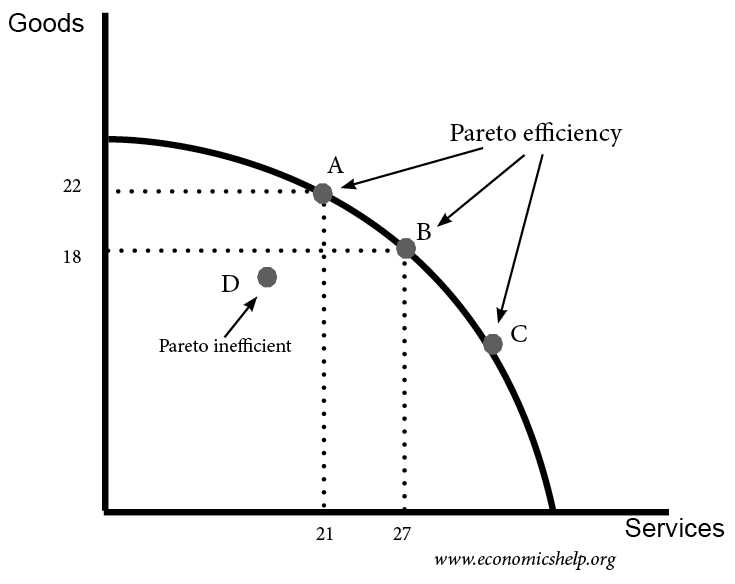
\includegraphics[width=0.8\textwidth]{ppf.png}
\end{figure}

\par{We can estimate the \ita{opportunity cost} of producing different goods by looking at the gradient of the line between the current point and the point we wish to investigate. The steeper the gradient (for greater $\Big|\frac{\mathrm{d}y}{\mathrm{d}x}\Big| $), the higher the opportunity cost}

\par{We can also look at the \ita{economic growth}. Economic growth means an expansion of the economy's production possibilities. Hence we should expect the graph to be scaled in all directions. This can come about due to an increase in the \ita{factors of production~\ref{model:prod}} (e.g. new hangar, whereby a company can produce more aircrafts of type A without reducing the number of type Bs). Or by advances in \ita{technology}(e.g. semicondutors industry, transistors, home pc)}

\defn{Factors of Production}{Any resource needed for the creation of a good or service (land, labor, capital and entrepreneurship)~\label{model:prod}}


\subsection{Comparative Advantage}

\par{The basic idea behind this model is that \ita{it makes sense to produce that which you're particularly good at producing, and buy that which you are not}. By choosing to produce the product (A) which as a lower opportunity-cost, the factors of production are freed from the other possible products. Hence this others can be obtained from trading with another entity which also benefits, since the product being traded has a higher opportunity-cost for them.~\ref{advantage}}

\defn{Comparative Advantage~\label{advantage}}{When an entity's opportunity-cost for some product is lower than that of some other entity's}

\begin{figure}[ht]
\centering
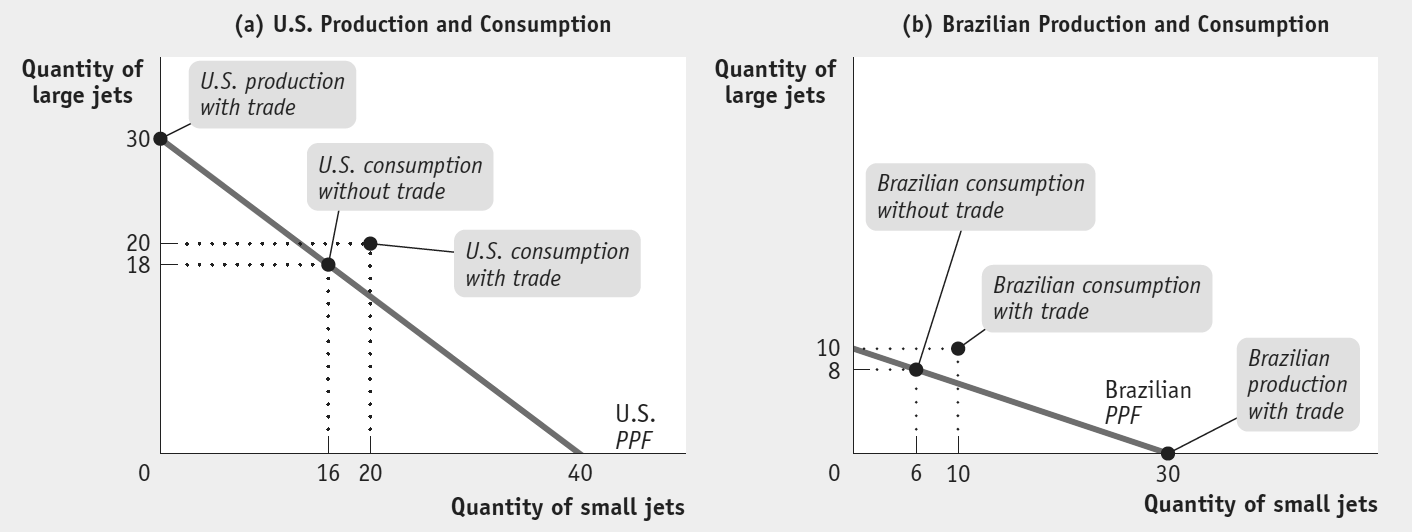
\includegraphics[width=0.9\textwidth]{jetsTrade.png}
\end{figure}

\rem{Note, how by trading, both production and consumption increase for both countries}

\defn{Absolute Advantage}{when an entity can produce more output per worker than other countries}

\par{Note that this doesn't mean that trading is no longer beneficial, what matters is the \ita{net gain}.It
does not matter whether it takes Brazil more resources than the United States to make a small jet; what matters for trade is that for Brazil the opportunity cost of a small jet is lower than the U.S. opportunity cost. So Brazil, despite its absolute
disadvantage, even in small jets, has a comparative advantage in the manufacture of small jets}

\begin{figure}[ht]
\centering
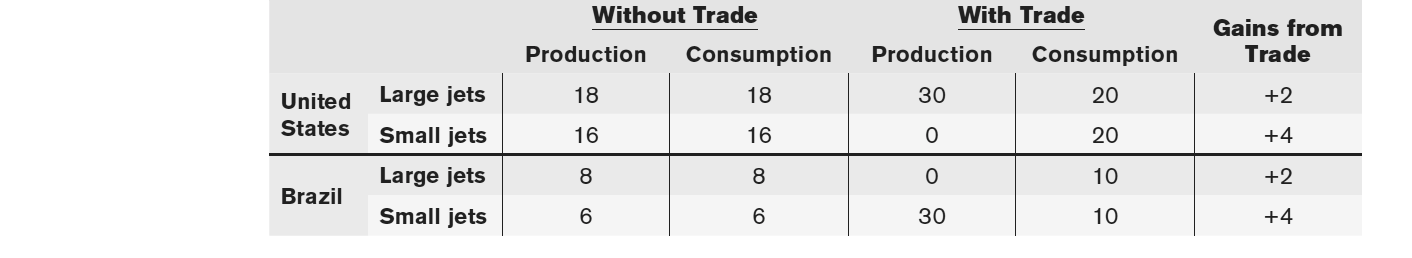
\includegraphics[width=0.9\textwidth]{jetsTrade2}
\end{figure}

\subsection{Interpreting the Simplification of Models}
\lecture{15}{01}{2019}
\par{The models used as examples above are grossly oversimplified, this of course has negative consequences, in particular makes the conclusions derived from them less reliable. Yet, as previously stated they are useful because they  illustrate best the fundamentals of economics.}

\par{The \ita{circular-flow diagram} for example, allow us to analyse the complex transactions that take place in an economy by looking at \ita{the flow of things}, and \ita{the flow of money}. The simplest of these has only 2 entities  \ref{flow:house} \ita{households} and \ref{flow:firms} \ita{firms}, whose interaction is mediated by two types of markets those for \ref{flow:goods} \ita{goods and services} and those for the \ref{flow:factor} \ita{factors of production}.}

\defn{Household~\label{flow:house}}{A person or group of people who share their income}
\defn{Firms~\label{flow:firms}}{An entity which produces goods and services}
\defn{Goods \& Services Market~\label{flow:goods}}{Where firms sell their products to households}
\defn{Factor Market~\label{flow:factor}}{Where firms buy the factors of production (e.g. job market)}
\newpage

\begin{figure}[ht]
\centering
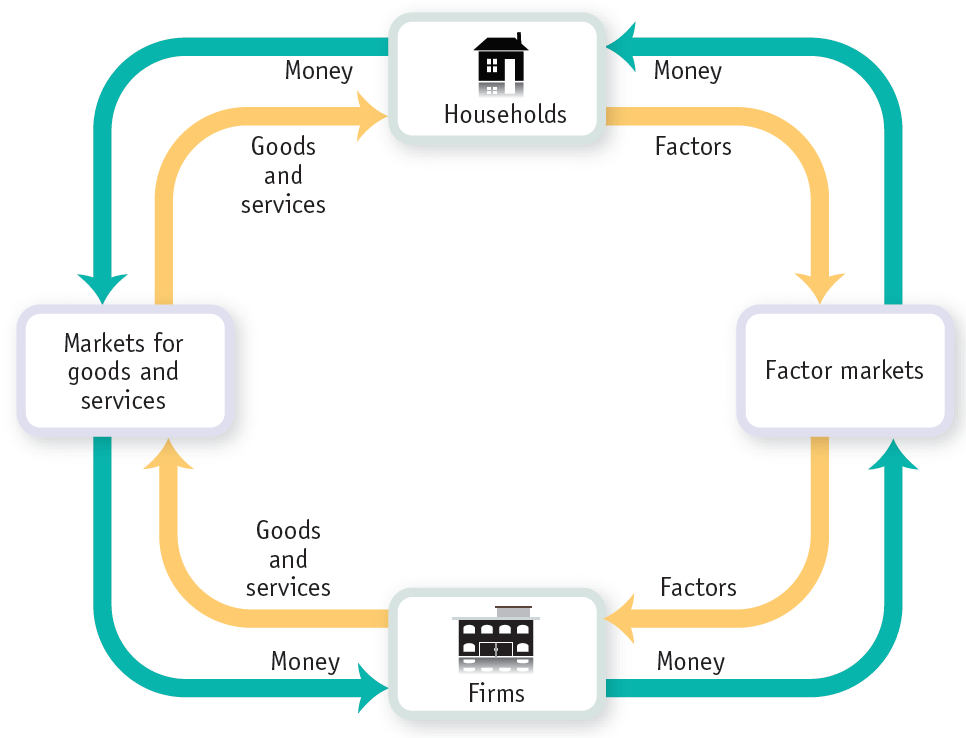
\includegraphics[width=0.7\textwidth]{flow.png}
\end{figure}

\rem{Note how the flows are opposite to each other, since \ita{in general} when an entity puts x into a system it gets y. As an illustration consider how the flow of money \ita{into} the market of goods \textbf{from} the household, leads to a flow of goods \ita{from} the market \textbf{into} the household.}

\par{We need to once again bear in mind the shortcomings of this model, for example the distinction between households and firms is not always clearly distinct, firms interact with each other and the government is not illustrated}

\subsection{Economic Analysis: Positive vs Normative}

\defn{Positive Economics}{Concerns itself with establishing matters of fact. It is therefore purely descriptive, it is able to provide right and wrong answers, but it does not pass any value judgments}

\defn{Normative Economics}{Prescriptive. It involves recommending courses of action to take in order to optimise an economy}

\rem{Note that even though positive economics deals with facts, and does not aim to prescribe behaviour, its conclusions can still be used to guide policy (e.g. politicians might enact certain policies based on forecasts)}

\rem{Even though there is no "right" answer \ita{per se} when it comes to normative economics, the reason it can still be used to guide public policy is because economists are able to agree on a certain course of action, regardless of their own personal values. Just like in ethics for example, where most scholars do not agree that there is one and one only way to live the \ita{good life} , yet most (if not all) agree that to kill an innocent child is morally blameworthy. In the realm of economics, think of two policies A and B  which achieve the same purpose, if A's net gains are higher then A is the right/preferable option. (e.g. rent control \& rent subsidies in the US)}

\newpage
\section{Supply and Demand}
\lecture{17}{01}{2019}
\subsection{Model of a Competitive Market}

\defn{Competitive Market}{A market where there exists many buyers and sellers, therefore none of them have the power to influence market prices}

\rem{Not all markets are competitive, if there are only a few major players, then they are able to set market prices}

\par{There are five key elements to the CM model}


\subsection{The Demand Curve}
	
	\par{The price of a product or service, affects the amount of that product that people will want to consume. In general, lower prices lead to higher demand~\ref{demand:law}. One can estimate the demand of a certain product by drawing out a table where we map the amount consumers would \ita{want} to buy for each price~\ref{demand:sch}. We can then observe how much would people be willing to pay for a certain quantity~\ref{demand:quantity}, it is by translating this information into a graph that we get the demand curve~\ref{demand:curve}}
	
	\defn{Law of Demand~\label{demand:law}}{A higher price for a good or service, \ita{other things equal}, leads people to demand a smaller quantity of that good or service}
	
	\defn{Demand Schedule~\label{demand:sch}}{How much of a good or service consumers will want to buy at different prices.}
	
	\defn{Quantity Demanded~\label{demand:quantity}}{actual amount of a good or service consumers are willing to buy at some specific price}
	
	\defn{Demand Curve~\label{demand:curve}}{a graphical representation of the demand schedule. It shows the relationship between quantity demanded and price}
	
	\rem{\textbf{N.B} It is paramount not to confuse quantity demanded with demand. Quantity demanded are the individual points on the demand curve}

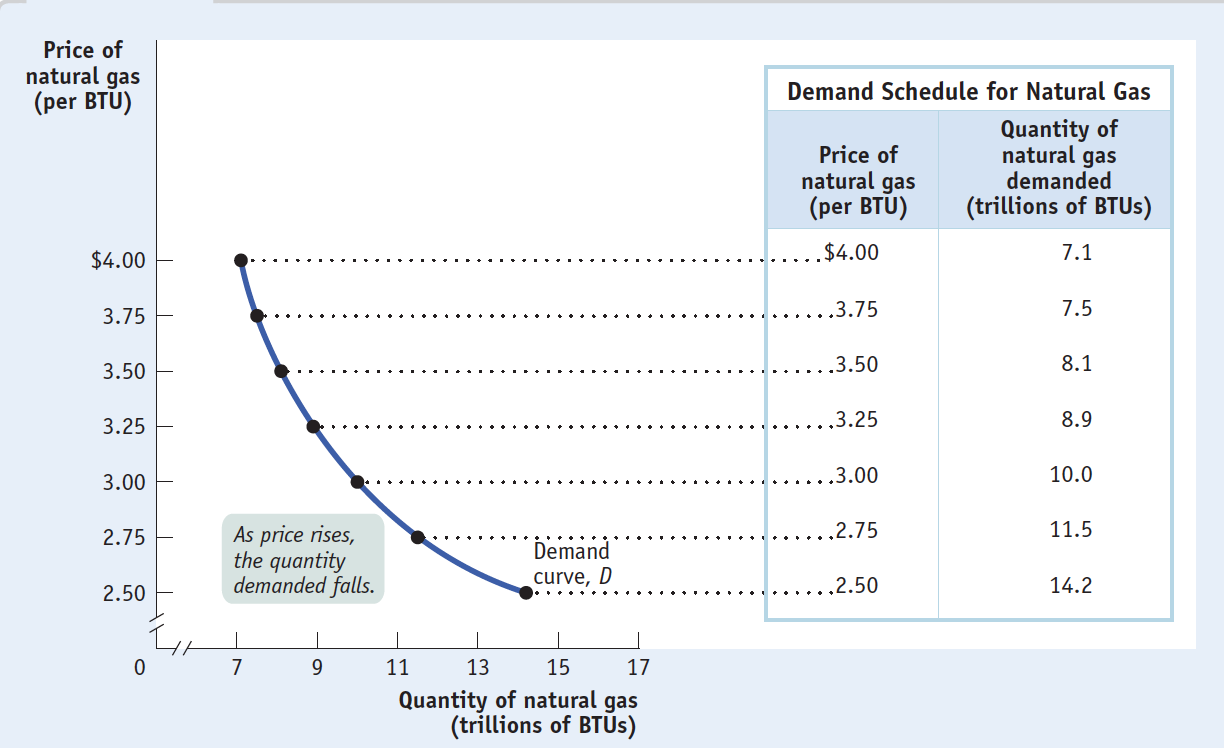
\includegraphics[width=15em]{demandCurve}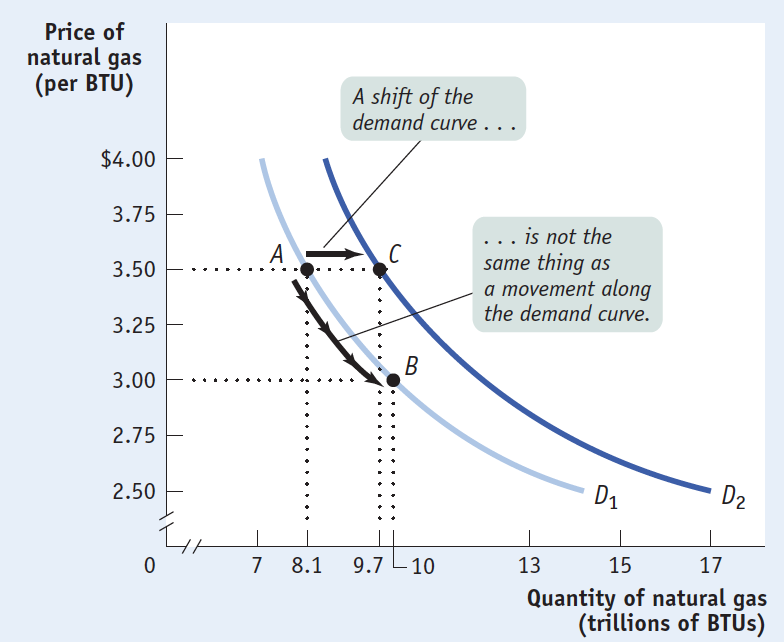
\includegraphics[width=15em]{demandShift}



		
	\par{One important distinction exemplified in the examples above is the graphical representation of a change in the market. We say that there is a shift in demand if \ita{for the same price, the quantity demanded increases}, hence this will translate into a horizontal translation of the curve. A shift of the quantity demanded simply moves us \ita{along the curve} (say for example if there's a sale). There are five major \textbf{non-price determinants} that can lead to a shift in demand:\mymarginpar{see 77 Table 3-1}}
	\begin{enumerate}
	\item  prices of related goods or services. 
	
	\defn{Substitute}{Two goods whose demand and price relation is proportional (price rise of coal leads to demand rise of solar panels)}
	\defn{Complement}{Two goods whose demand and price relation is inversely proportional (increased price of coffee decreased cookie consumption)}
	
	\item income
	
	\defn{Normal Good}{goods whose demand increases, when income increases (holidays)}
	\defn{Inferior Good}{goods whose demand decreases, when income decreases (bus tickets)}
	
	
	\item tastes
	\item expectations
	
	\item number of consumers
	
	\defn{Individual Demand Curve}{illustrates the relationship between quantity demanded and price for an individual consumer.} 
	
	\par{The market demand curve is obtained by performing the horizontal sum of the total number of consumers. If the number of consumers grow and the price remains unchanged, then an increase in demand is necessary.}
		\begin{figure}[ht]
\centering
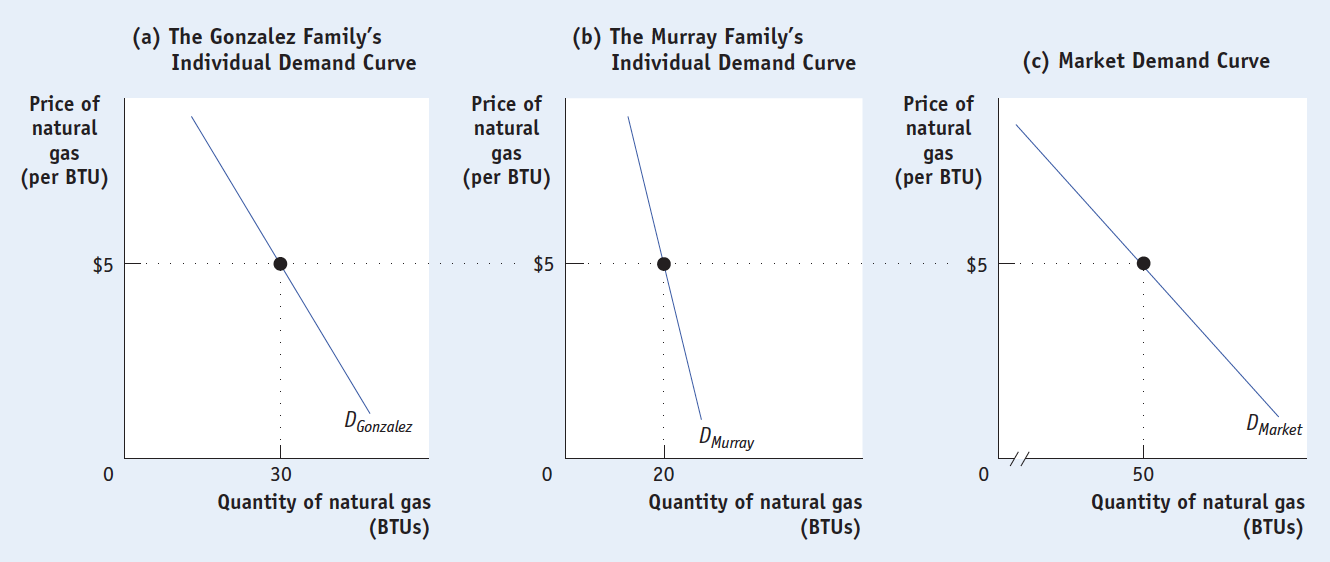
\includegraphics[width=\textwidth]{demandIndividual}
\end{figure}

	\end{enumerate}
	
	
		
\subsection{Supply Curve}

\lecture{18}{01}{2019}

\par{By considering the production of goods, instead of their consumption/demand, we get the analogous supply curve. Note that while the demand curve is in general decreasing (lower price $\implies$ more consumption), the supply curve is generally increasing. This makes sense, as \ita{all things equal}, higher pricers translate into higher profits}

\defn{Quantity Supplied}{Actual amount a producer would be willing to sell their products for a specific price}

\defn{Supply Schedule}{How much of a good or service producers will want to sell at different prices}

\defn{Supply Curve}{Graphical representation of the relation between quantity supplied and price}



\begin{figure}[ht]
\centering
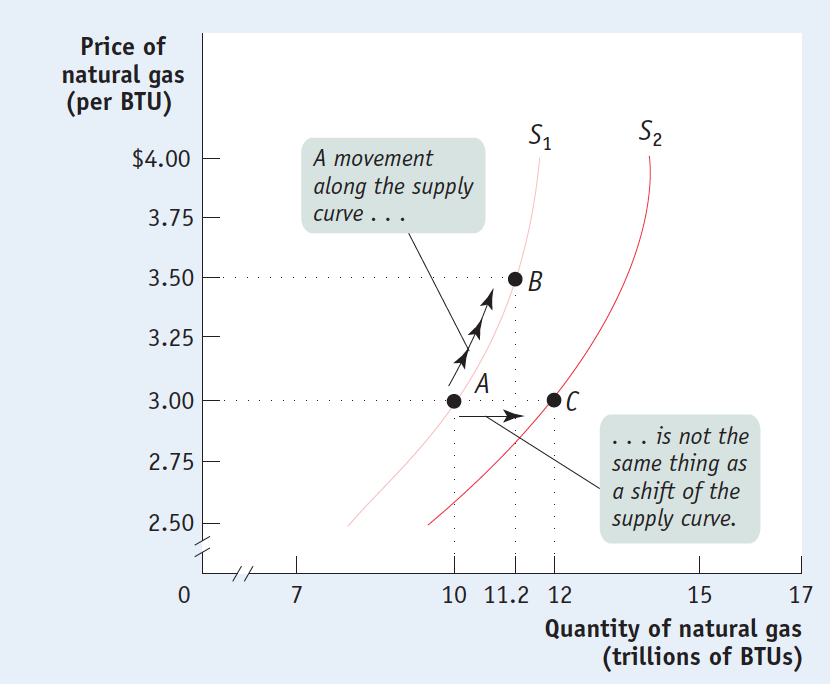
\includegraphics[width=0.5\textwidth]{supplyCurve}
\end{figure}

\par{Note that just like when looking at the demand curve, it's important not to confuse quantity supplied with supply, and their corresponding changes; a movement along the supply curve (increase in q.s) and a shift of the whole curve (increase in supply). The five major causes of a change in supply are due to changes in one or more of the following \textbf{non-price determinants}:}

\begin{enumerate}
	\item Input prices
	
	\defn{input}{good or service used to produce other goods/services}
	
	\par{The supply curve shifts inversely to the price of inputs, i.e. if an input becomes costlier, there's a reduction in supply $=$ shift to the left, and vice-versa}
	
	\item Prices of related goods or service
	
	\par{An increase in the price of a \ita{substitute} product will lead to a decrease in supply of its "pair" product. The reverse is true for its \ita{complement}.}
	
	\ex{If a company sells products A,B which serve roughly the same purpose, an increase of the price of A will make it more profitable, hence the company will decide to allocate more resources to A and decrease supply of B}

	\item Technology
	
	\par{Technological advancements lead to a decreased input cost, which in turn decreases the total cost of production leading to an increase in supply}
	
	\item Expectations
	
	\par{A producer may decide to store part of its goods to sell at a latter date, when demand is expected to be higher. This choice depends on a comparison of the current price versus the expected future price}
	
	\item Number of producers
	
	\par{Just like with the individual demand curve, if there are several producers of the same type of good, the supply curve will be equal to the horizontal sum of each producer's individual curve}
	
	\begin{figure}[ht]
\centering
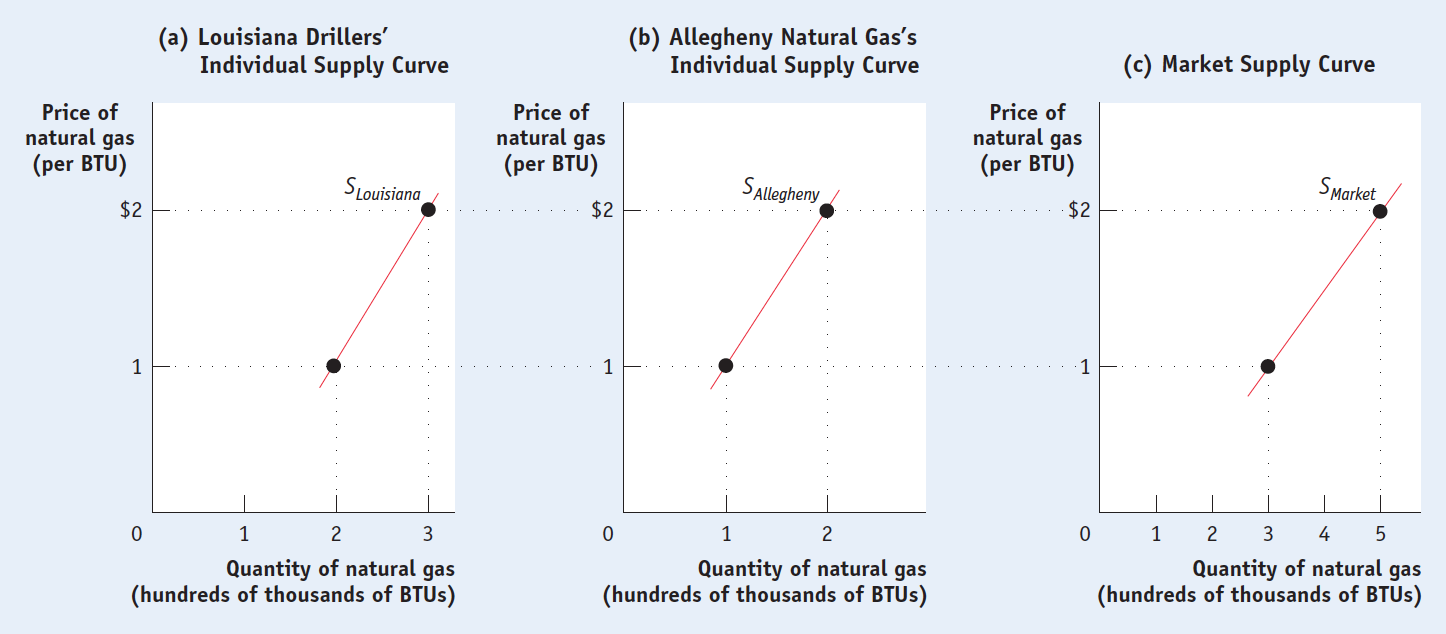
\includegraphics[width=0.5\textwidth]{supplyIndividual}
\end{figure}

\end{enumerate}

\subsubsection{Equilibrium}


\defn{Equilibrium Price*~\mymarginpar{*market clearing price}}{The price where the quantity demanded and supplied match.}

\rem{This is easily observed by finding the intersection of the supply and demand curves}

\par{In general, the market price will tend towards an equilibrium due to the following:}

\begin{enumerate}

\item Homogeneity

	\par{Given that both buyers and sellers are well informed of the "normal" prices in a certain area for a certain product, consumers will look for the cheaper products which achieve the same, or similar end. Sellers must have competitive prices (too low $\implies$ profit loss ; too high $\implies$ costumers loss)}
	
\item Price Fall

	\par{If the prices are set above that of the equilibrium, there will be a \ita{surplus} of goods. The market will adjust, by lowering the price towards eq}
	
	\defn{Surplus}{Quantity demanded $<$ Quantity Supplied}
	
\item Price Rise

	\par{If the prices are set below that of the equilibrium, there will be a \ita{shortage} of goods. The market will adjust, by raising the prices towards eq. so that quantity demanded is lowered}
	
\end{enumerate}


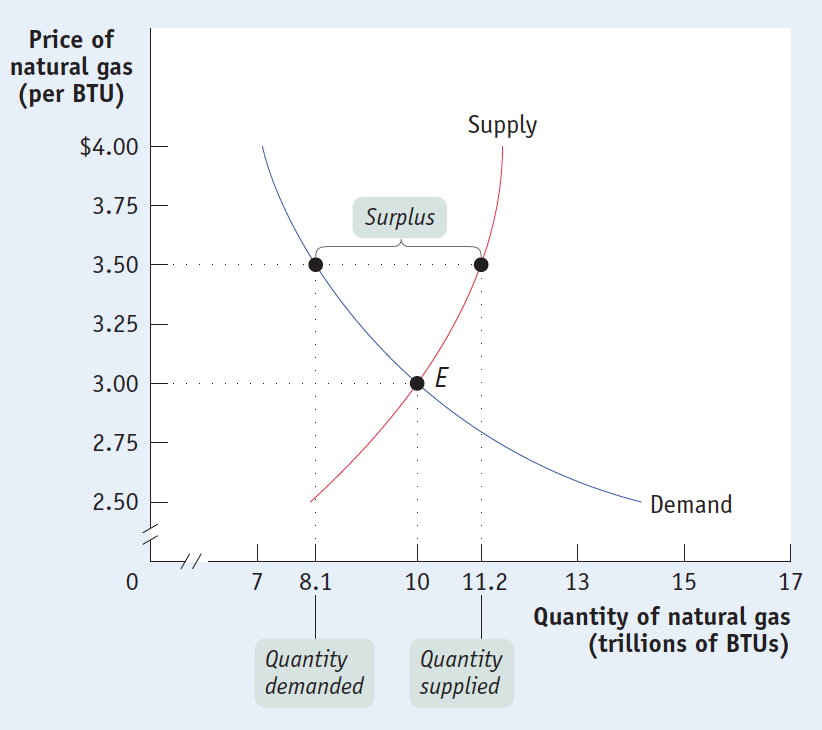
\includegraphics[width=15em]{supplySurplus}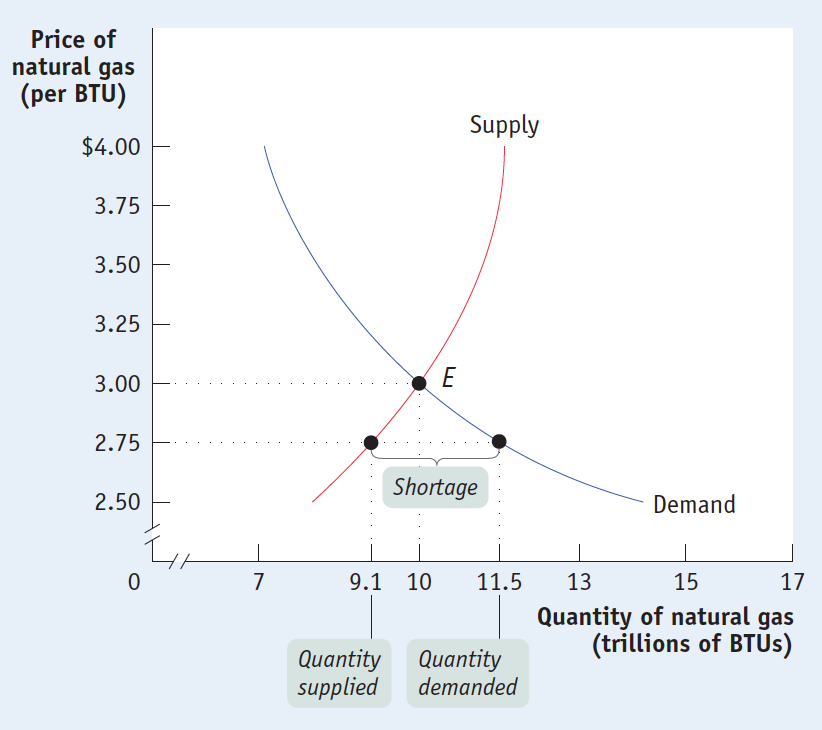
\includegraphics[width=15em]{supplyShortage}


	\par{Considering what happens to the equilibrium point when changes in supply and demand occur, one finds that:}
	
	\defn{Shortage}{Quantity Demanded $>$ Quantity Supplied}
	\begin{enumerate}
		\item An increase in demand leads to an upward movement along the supply curve, i.e. both the price and quantity demanded increase*~\mymarginpar{and vice-versa}
		\item An increase in supply leads to a downward movement along the demand curve, i.e. the price decreases while the demand increases*
	\end{enumerate}
	
	\rem{When there's a shift in both the demand and supply, if the price and quantity of equilibrium move together, then this is due do a change in demand. When they move in opposite directions, then it is due to a change in supply}

\begin{figure}[ht]
\centering
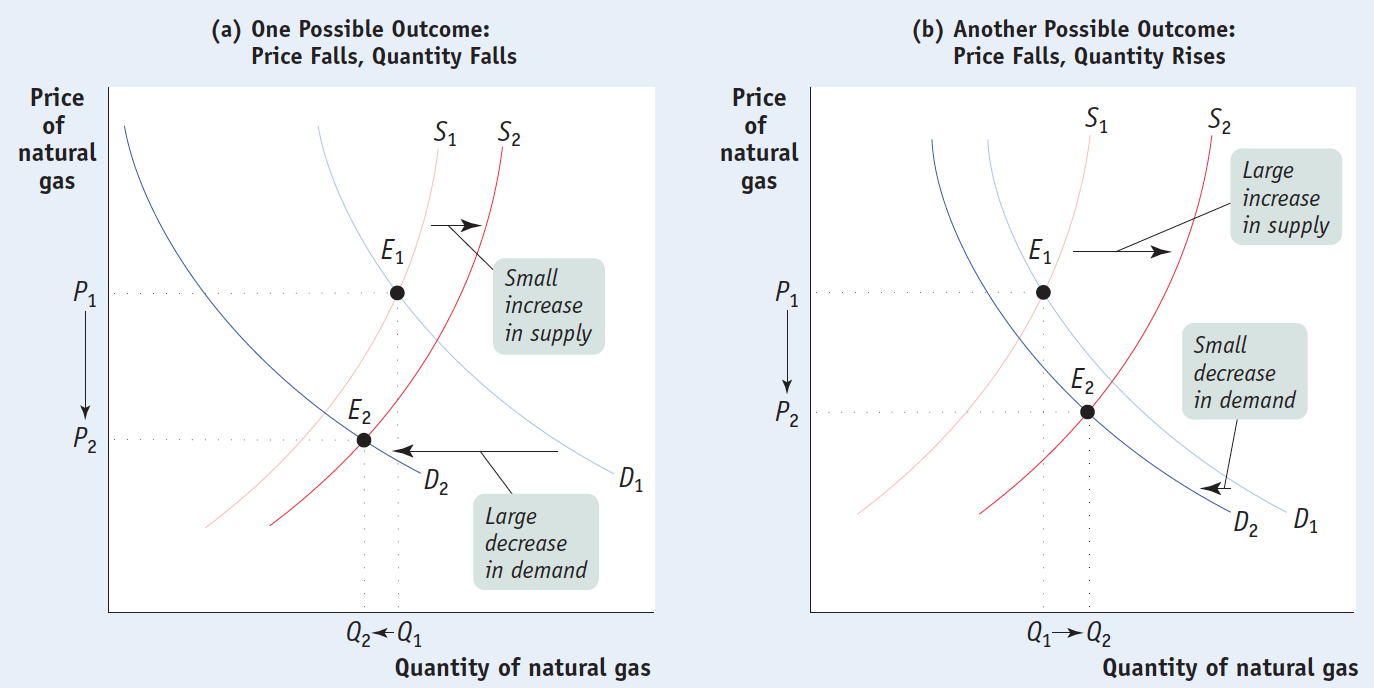
\includegraphics[width=\textwidth]{supplydemandEq}
\end{figure}

\newpage
\section{Consumer and Producer Surplus}

\lecture{22}{01}{2019}
\subsection{Consumer}

\defn{Willingness to Pay}{maximum price at which the buyer would buy the good}

\defn{Individual Consumer Surplus}{net gain to an individual buyer from a purchase}

\nota{  S = Willing - Actual}

\defn{Total Consumer Surplus}{net gain of all individuals}

\rem{Economists use consumer plus to mean both total and individual, it can be differentiated from context}


\begin{figure}[ht]
\centering
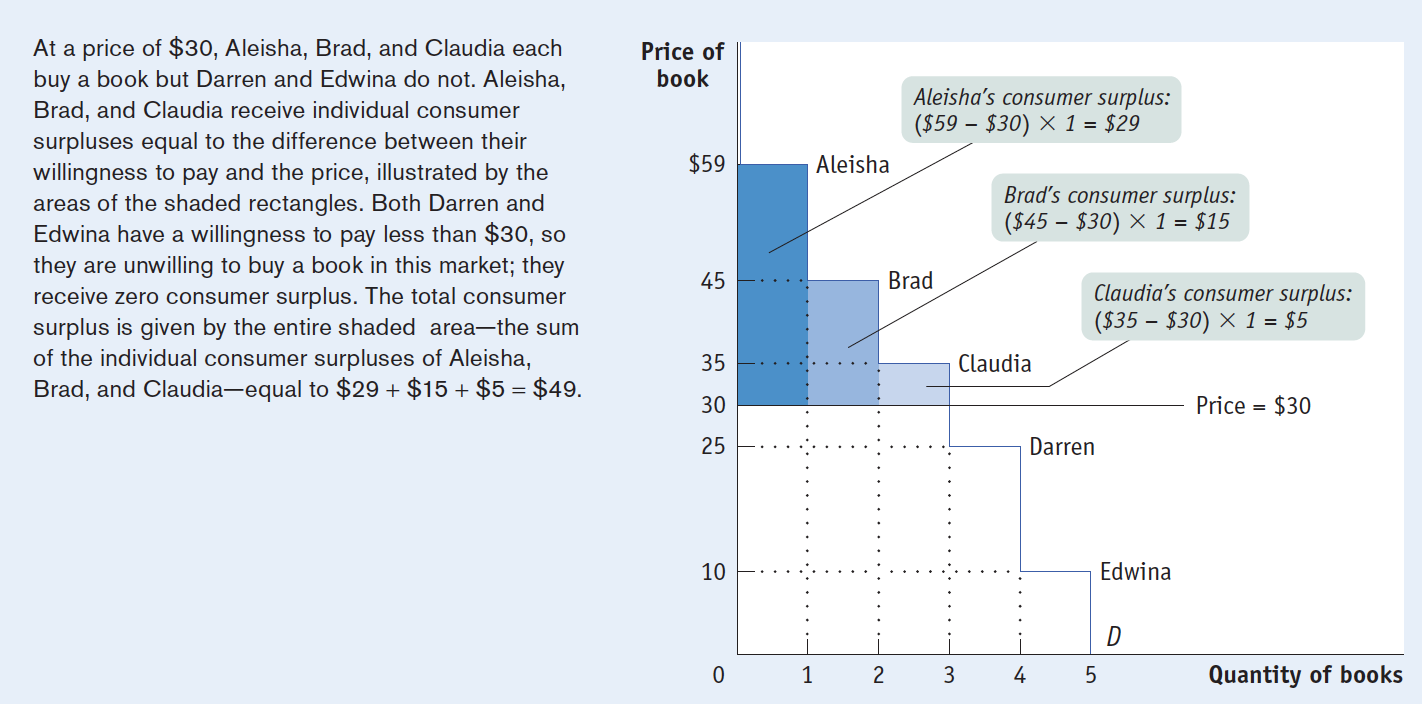
\includegraphics[width=0.7\textwidth]{consumerSurplus}
\end{figure}

\rem{It is intuitively obvious, that a change in market price varies inversely with consumer surplus}

\subsection{Producer}

\par{The producer surplus works much in the same way, but in reverse. The gains for sellers are calculated by looking at the difference between the min price a seller would be willing to sell his products/goods and the actual price it was sold}

\defn{Cost}{the lowest price at which he or she is willing to sell a good}

\defn{Individual Producer Surplus}{net gain to an individual producer from a sale}

\defn{Total Producer Surplus}{net gain of all individual producers}

\begin{figure}[ht]
\centering
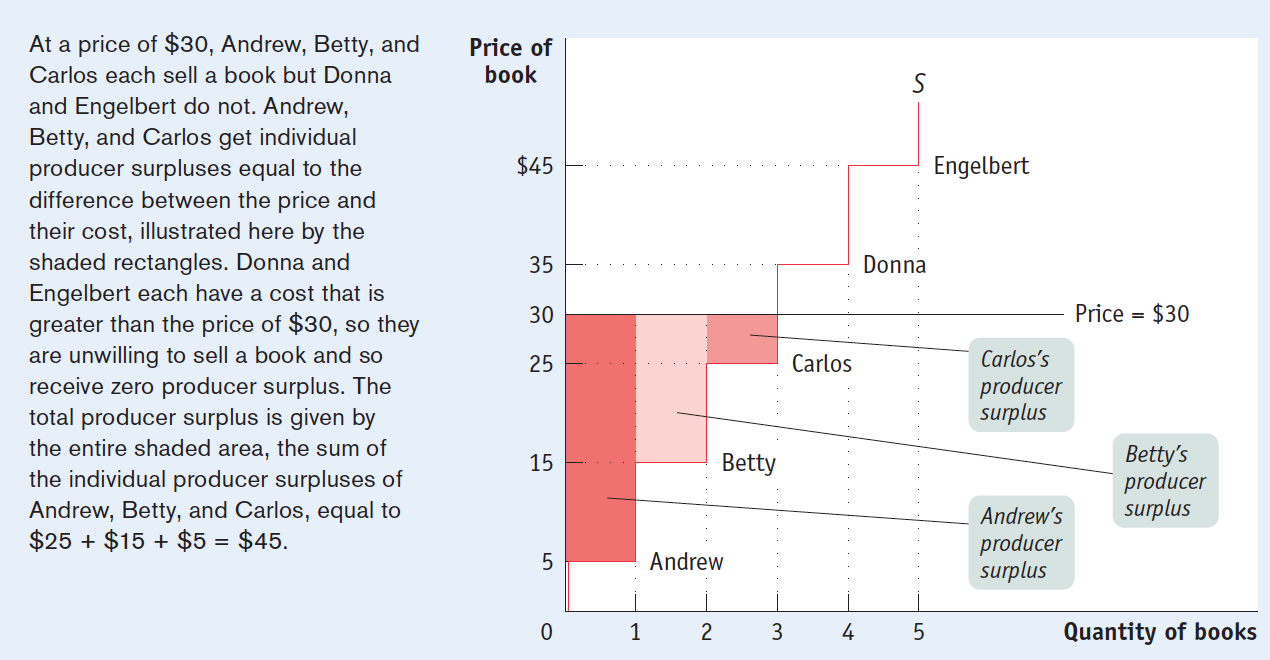
\includegraphics[width=0.7\textwidth]{producerSurplus}
\end{figure}

\rem{Once again it should be obvious that if the market price increases the producer surplus will also increase}

\par{By looking at the net gains generated for both producers and consumers we can calculate the total surplus for a market. This is evidence that trade can be beneficial for both}

\defn{Total Surplus}{the sum of the producer and consumer surplus}

\begin{figure}[ht]
\centering
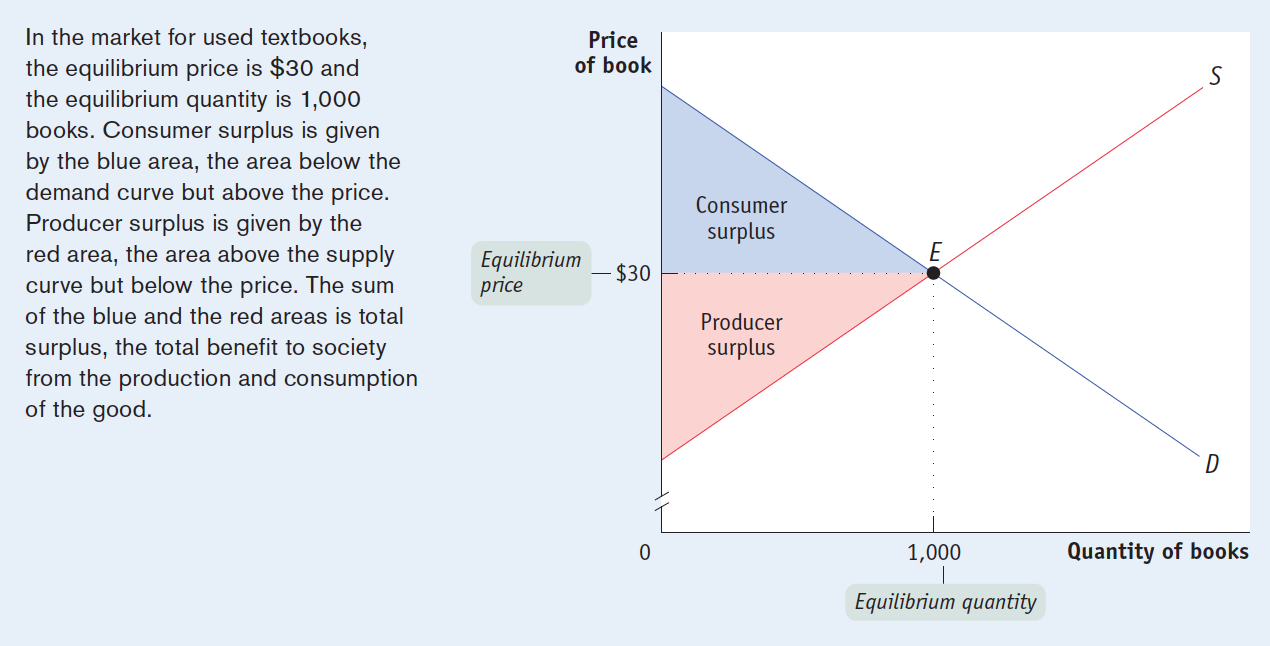
\includegraphics[width=0.7\textwidth]{CPsurplus}
\end{figure}


\rem{The surplus is the area found below (producer) and above (consumer) the equilibrium price}


\subsection{Efficiency}


\par{We can analyse the efficiency of a market in the light of consumer and producer surplus. Say for example that one is aiming to improve the market equilibrium by increasing total surplus. How could this be achieved? In essence an efficient market performs the following four functions:}

\begin{enumerate}
	\item It Allocates consumption of the good to the potential buyers who have the highest willingness to pay.
	
	\item  It allocates sales to the potential sellers who most value the right to sell the good, as indicated by the fact that they have the lowest cost.
	
	\item It ensures that every consumer who makes a purchase values the good more than every seller who makes a sale, so that all transactions are mutually beneficial.
	
	\item It ensures that every potential buyer who doesn't make a purchase values the good less than every potential seller who doesn't make a sale, so that no mutually beneficial transactions are missed.
\end{enumerate}

\par{In general, \ita{any way of allocating the good other than the market equilibrium outcome lowers total surplus}. There is however things one must watch out for when relying purely on markets.}

\begin{enumerate}
	\item Equity/Fairness is often in conflict with efficiency: As a society we often don't think as efficiency as the only goal to be achieved, in fact most modern societies understand the trade-off between the two, and often prize the distribution of wealth over the maximisation of efficiency. The reason why this two conflict is that efficiency deals only with maximising a the output of a function given certain inputs, once the output/goal being optimised is defined that's what the optimising strategies will work to increase regardless of what extraneous consequences it might have
	
	\item Markets Fail: 
		\begin{itemize}
		\item in an attempt to capture more surplus, one party prevents mutually beneficial trades from occurring (monopoly)
		\item actions of individuals sometimes have side effects*~\mymarginpar{externalities e.g. pollution} on the welfare of others that markets don't take into account
		\item Markets for some goods fail because these goods, by their very nature, are unsuited for efficient management by markets. (e.g. problems of private information - used car)
		\end{itemize}
		
	\item Even when the market equilibrium maximizes total surplus, this does not mean that it results in the best outcome for every individual consumer and produce
\end{enumerate}

\par{When markets are efficient, the economy as a whole is efficient. Even though economies where every market is efficient are a theoretical construct, some are much more efficient than others. Why is that? It all comes down to two main market features (1) Property Rights; (2) Prices as Economic Signals }

\defn{Property Rights}{system in which valuable items in the economy have specific owners who can dispose of them as they choose}

\par{By taking ownership full ownership of goods once bought, this reduces the opportunity-cost of the item. For example, by knowing in advance that I might be able to sellback a textbook which I only need for a semester, I will in recoup part of its original cost, and the student buying it will not only be able to buy it at a reduced cost, but will also gains the right to resell it} 

\defn{Economic Signals}{any piece of information that helps people and businesses make better economic decisions}

\par{Business analysts often know that a business is preparing to ramp production when it increases its purchase of cardboard boxes, we say that the boxes are a signal of changes in industrial production. In a more general case, prices in a market economy perform a similar function. By setting the market price of a good at $x$ , economic agents can derive useful information from  it. Sellers know that there are consumers willing to pay at least $x$, and consumers know that there are potential sellers with a cost of $x$ or less. The signal given by the market price ensures that total surplus is maximized by telling people whether to buy, sell , or do nothing at all.}

\rem{ Note that since, in equilibrium, the quantity demanded equals the quantity supplied, all willing consumers will find willing sellers.}

\rem{There are markets where prices are not a good economic signal, for example when there is uncertainty about the quality of a good. This is a well-known problem in economics know as \ita{"the market for lemons"}}

\section{Meddling with Markets}

\lecture{24}{01}{2019}

\par{There is often the need for the government to implement price controls, this can come in the form of price floors or price ceiling}

\subsection{Price Ceiling}

\defn{Price Ceiling}{government mandated maximum price at which a good can be sold}

\par{Price ceilings are often set in place during times of crises, where demand for certain goods sky-rockets, and producers tend to take advantage of the situation by charging way above market-price. However, when balanced markets are over-regulated predictable negative consequences arise, the main one being that producers seeing their profit margins decline tend to reduce supply, which leads to shortages. }

\rem{If the price ceiling is set above market price, we say that it is \ita{non-binding}, i.e. it will not constraint market behaviour}

\begin{figure}[ht]
\centering
\includegraphics[height=0.3\textwidth, width=0.5\textwidth]{ceilling}
\end{figure}


\begin{itemize}
	\item \textbf{Negative Consequences}
	\begin{enumerate}
		\item Low Quantity: given that producers will produce less, it necessarily follows that consumers will buy less. This mutual loss is called \ita{deadweight loss}, it represents the reduction in the total surplus.
		
		\defn{deadweight loss}{the loss in total surplus that occurs whenever an action or a policy reduces the quantity transacted below the efficient market equilibrium quantity}
		
		\begin{figure}[h]
\centering
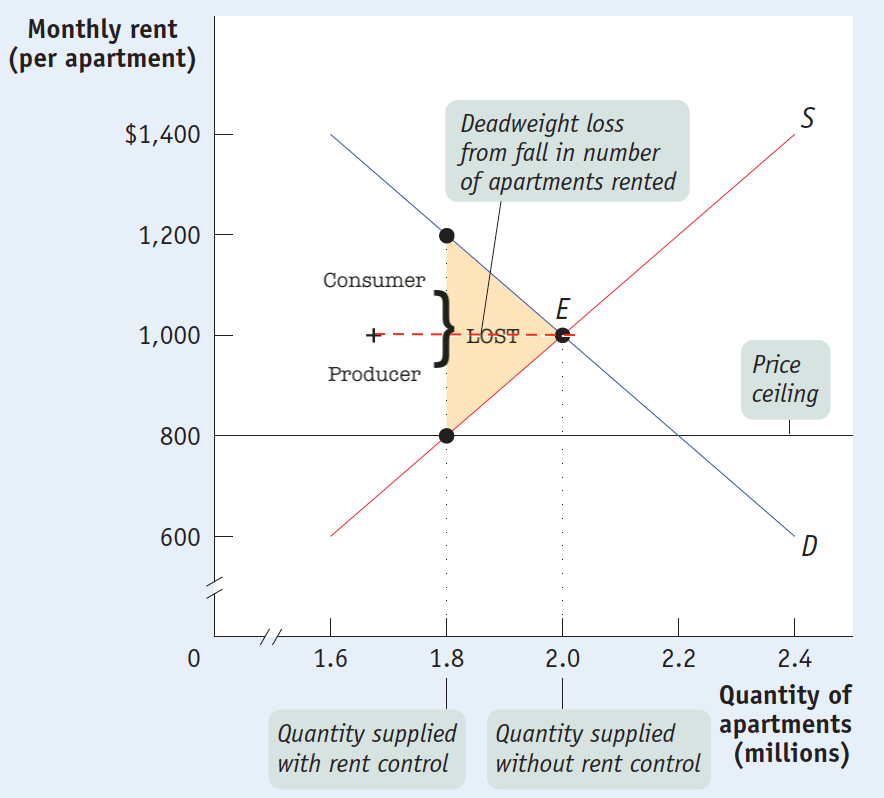
\includegraphics[height=0.4\textwidth,width=0.8\textwidth]{deadweight}
\end{figure}
\begin{figure}[h]
\centering
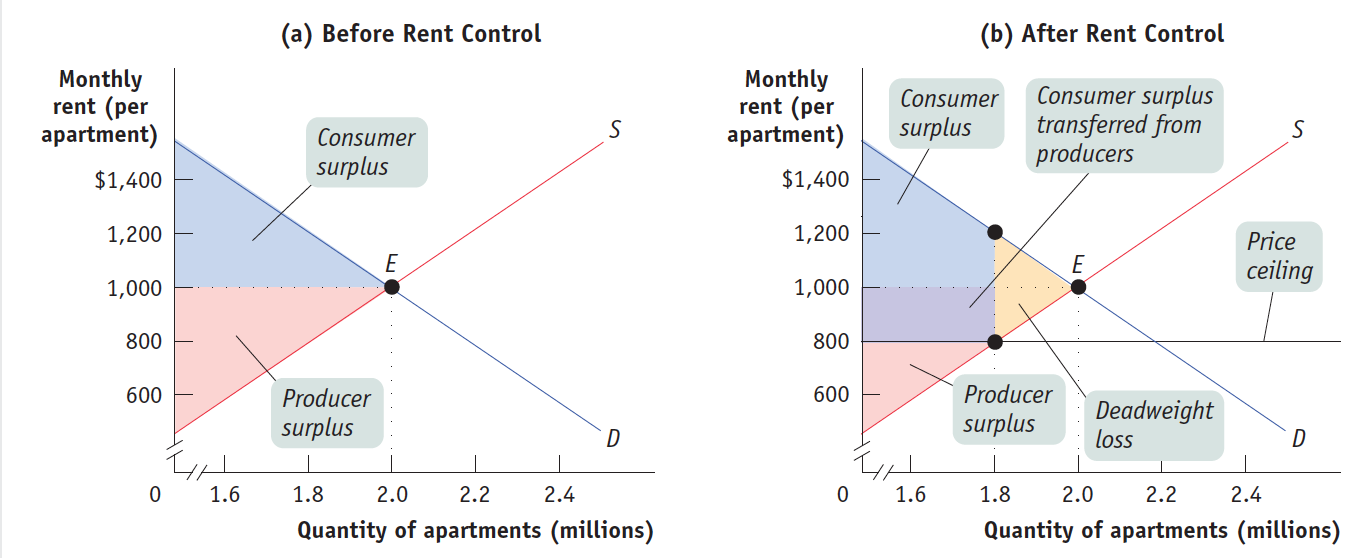
\includegraphics[height=0.4\textwidth,width=0.8\textwidth]{deadweight2}
\end{figure}
	
	\item Allocation to Consumers: apartment, some want one badly and are willing to pay a high price to get it. Others have a less urgent need and are only willing to pay a low price~\mymarginpar{Krugman correlates willing max price to urgency/necessity, but it doesn't necessarily follow! One might be in dire need of a house, but simply not be able to afford to go any higher}. By "lowering the bar" for everyone, other factors other than price (personal connections, luck) will take over the allocation, which often turns out to be inneficient
		
	\item Wasted Resources: people expend money, effort, and time to cope with the shortages caused by the price ceiling
	
	\item Low Quality: sellers offer low-quality goods at a low price even though buyers would rather have higher quality and would be willing to pay a higher price for it
	
	\item Black Markets
	
	\end{enumerate}
	
	\item \textbf{Why are ceilings needed?} \par{they give a small minority
of buyer much cheaper products than they would get in an unregulated market, which they wouldn't otherwise be able to afford}

\end{itemize}

\subsection{Price Floors}


\defn{Price Floor}{government mandated minimum price at which a good can be sold (e.g. min wage)}

\par{Price floors are often set in place as an aid to highly competitive  markets (e.g. job market, farming), where supply for certain goods is plenty.}

\begin{figure}[h]
\centering
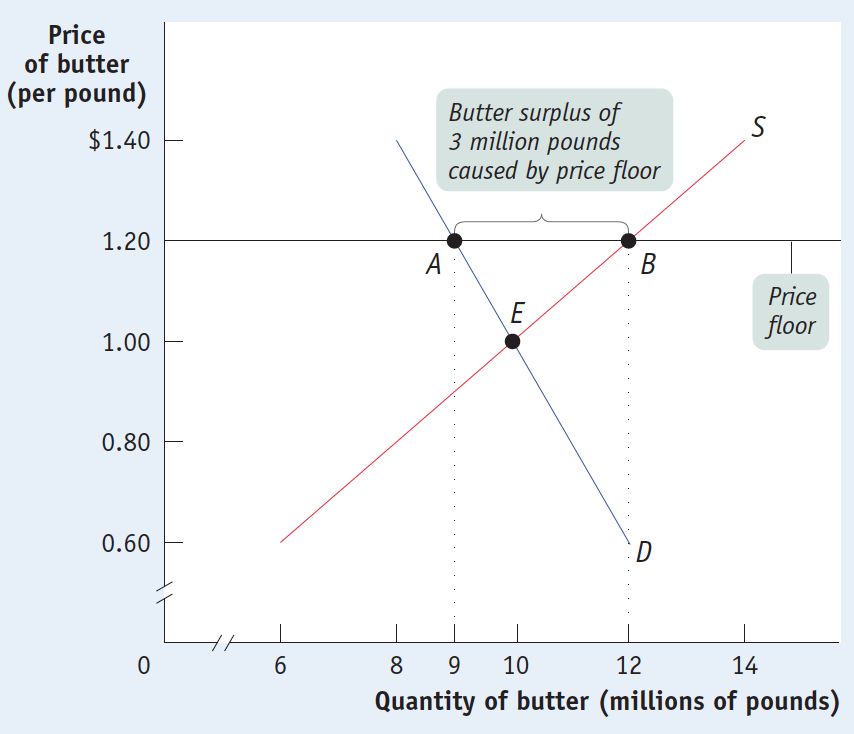
\includegraphics[width=0.5\textwidth]{floor}
\end{figure}

\rem{Both ceilings and floors have the effect of reducing the quantity of a good bought and sold. When the quantity of a
good supplied isn't equal to the quantity demanded, \textbf{the actual quantity sold is determined by the "short side" of the
market (whichever quantity is less)}. Sellers don't want to sell as much as buyers want to buy, it's the sellers who determine the actual quantity sold. If buyers don't want to buy as much as sellers want to sell, it's the buyers who determine the actual quantity sold}

\rem{The negative side effects are similar to those of price floors}

\subsection{Controlling Quantities}
\lecture{25}{01}{2019}

\par{Until now we have been focusing on government intervention on the prices of goods, in this section we'll focus on controlling quantities}

\defn{Quota}{an upper limit on the quantity of
some good that can be bought or
sold.}

\defn{Quota Limit}{the total amount of the good
that can be legally transacted}

\rem{This limits are usually enacted by issuing licenses, which limits the number of people which can sell the good}

\defn{Demand Price}{the price at which
consumers will demand that quantity.}

\defn{Supply Price}{the price at which producers will
supply that quantity.}

\par{Licenses are not free, the owner of a licence must buy it from the local council, which makes it in itself a commodity separate of the good. Therefore, when analysing transactions one must consider two distinct (but related) markets (1) the transactions between customer-seller (2) transactions of licenses.}
\par{Given that this cost of the license is usually carried over to customers, there is a a difference between what  customers pay and the profit the seller does, this difference can be see as the license fee which belongs to the license holder who usually leases it}

\defn{wedge}{a difference between the demand price
and the supply price of a good; that
is, the price paid by buyers ends up
being higher than that received by
sellers.}

\defn{quota rent}{the earnings that
accrue to the license-holder from
ownership of the right to sell the
good. It is equal to the market price
of the license when the licenses are
traded.}

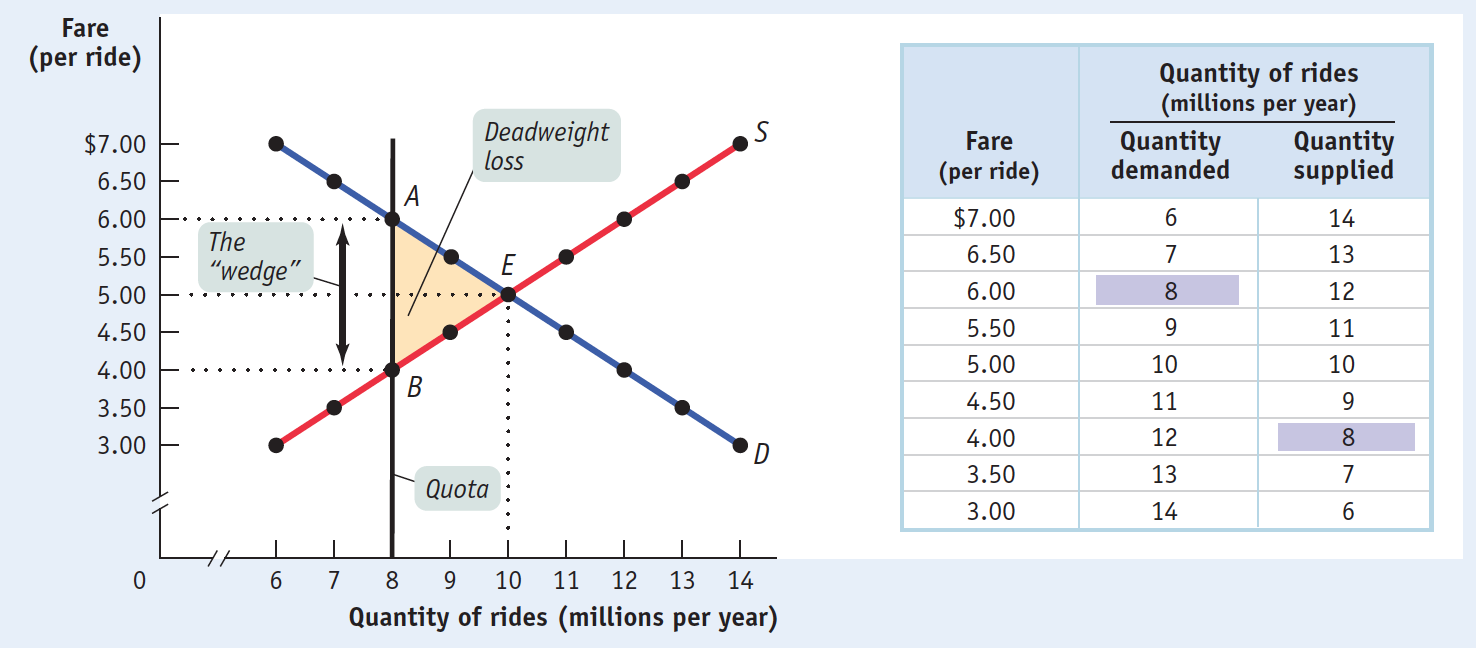
\includegraphics[width=\textwidth]{control}

\newpage

\section{Elasticity}


\defn{Elasticity}{a measure of a variable's sensitivity to a change in another variable}

\defn{Price Elasticity of Demand}{change in the quantity demanded in relation to a price change}

$$ PED = \left|\frac{\% \ \Delta QD}{\% \ \Delta P} \right|$$

\rem{remember to change the change to a percent value}

\rem{Due to (\ref{demand:law}) , the value will always be negative, indicating that QD and P vary inversely. By convention the sign is dropped}

\defn{Elastic}{A product $P$ is deemed to be elastic, if its $PED < 1$; i.e if the change in price is greater than the change of the quantity demanded}

\defn{Inelastic}{$PED > 1$; change of qd is greater than price change}

\defn{Unit Elastic}{$PED = 1$}

\par{\textbf{The Midpoint Method} is used , instead of the method above, to avoid computing different elasticities for different pov's. For example, John is 180cm tall and Mary is 162cm tall. From John's perspective, their percentual difference is 110\% while from Mary's is 90\%} \TODO{Ask! if they vary by 10, when using the words taller/shorter than this is assumed. So why is it necessary}

\par{The concept is still the same but the change of the variables is divided by its average}
\ex{
$$ \% \Delta QD = \frac{QD_2 - QD1}{\sfrac{(QD_2 + QD_1)}{2}}$$
}

\par{In general:}

$$ \% PED = \frac{\tfrac{QD_2 - QD1}{\sfrac{(QD_2 + QD_1)}{2}}}{\tfrac{P_2 - P1}{\sfrac{(P_2 + P_1)}{2}}}$$

\subsection{Interpreting PED}

\defn{Perfectly Inelastic}{changes in price do not affect the quantity demanded}

\par{Note that in the case where customers do not respond to changes in price (e.g. serious chronic disease medication), the demand curve will in fact just be a vertical line, since $\Delta QD = 0$}

\defn{Perfectly Elastic}{changes in demand do not affect price}

\par{Note that in the case where \ita{any} price change leads to extreme changes in the quantity demanded*\mymarginpar{*real life scenarios are scarce, but a close example would be of two products which are really good substitutes of each other}, the demand curve will then be an horizontal line, since for $+\Delta P , \Delta Q \to 0$ and  $-\Delta P, \Delta Q \to \infty$} \TODO{ASK! Should there not be two asymptotes instead of a horizontal line?}

\rem{Note then that in general, since we represent price in the $y$ axes and qd in the $x$ axes, $PED = \frac{1}{\frac{dy}{dx}}$ , it follows then that the steeper the gradient , the less elastic a product is}


              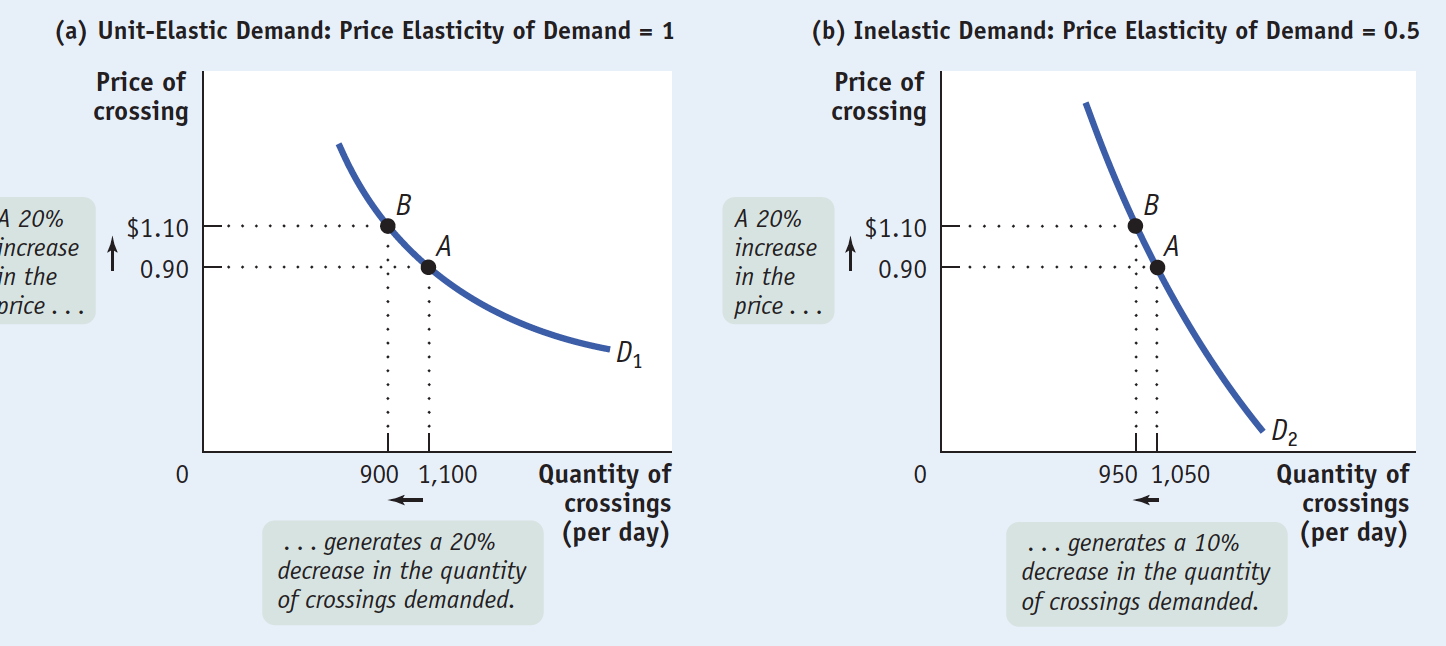
\includegraphics[width=0.65\linewidth]{elasticGrad} 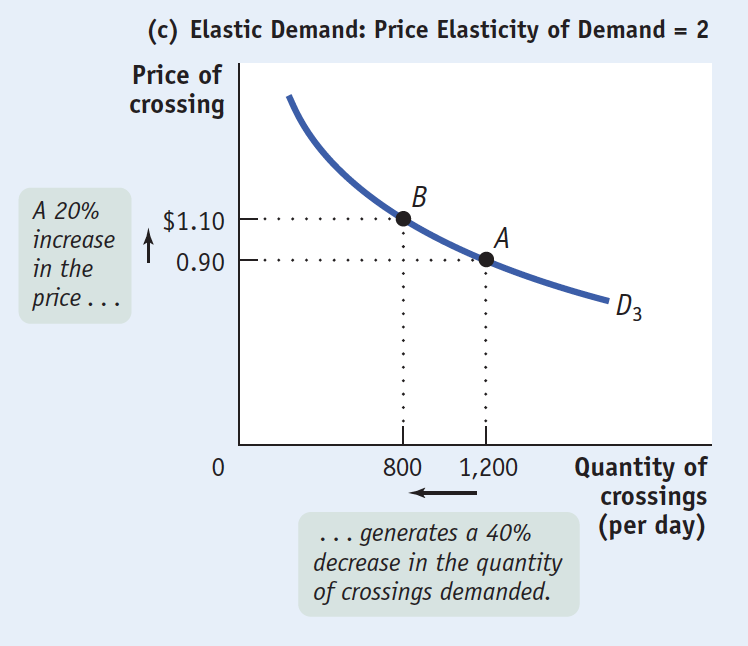
\includegraphics[width=0.335\linewidth]{elasticGrad2}

\par{The notion of elasticity is obviously useful to predict how of possible changes in price will affect the \ita{total revenue}.}

\defn{Total Revenue}{the total value of sales of a good, equal to the price multiplied by the quantity sold}

$$T_n = P_n \cdot Q_n$$ 

\par{where $T_n$ represents the total revenue of a good at the point $(Q_n,P_n)$ in the demand curve}\\

\par{The total revenue after a change can still be calculated in the same way. We should expect the area to change due to the (1) price effect ; (2) demand effect. It should be intuitively obvious that by raising the price the p/product revenue will be higher, and the opposite is true when reducing quantities. However, the elasticity of the curve is useful to help us understand which of these effects will be stronger, and in turn what happens to the \ita{net total revenue}}

\par{It is useful again to think of the gradient of the curve and the area of the rectangle strictly below the point we're looking at. Note the following for a price increase along the curve\mymarginpar{obviously the opposite is true for a decrease}:} 

\begin{itemize}
	\item{\textbf{Elastic:} for a steeper gradient, even a small decrease in qd will result in a very large increase in price (think of an exponential curve). Hence, \textbf{the revenue lost by the lost units will be compensated by the revenue gained by the increase in price}}
	\item{ \textbf{Non-Elastic:} the opposite}
	\item{ \textbf{Unit-Elastic:} still no change}
\end{itemize}

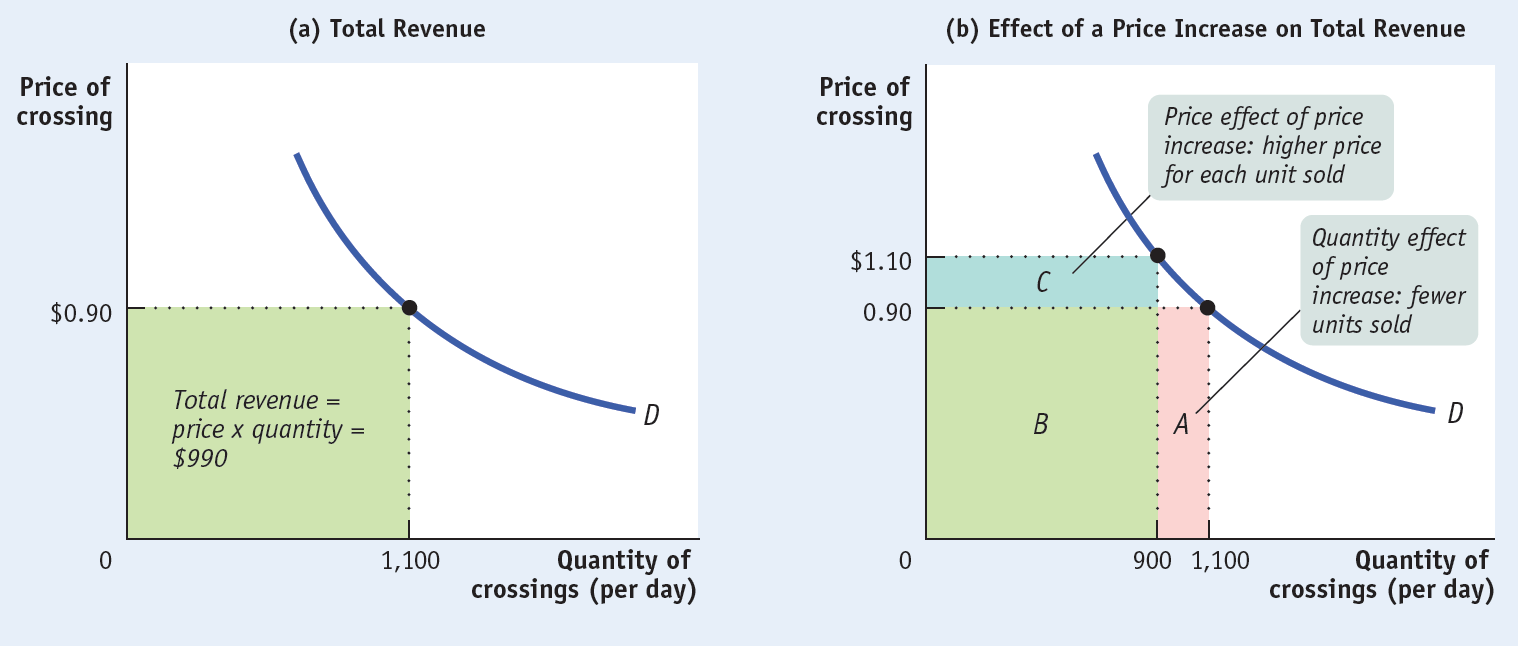
\includegraphics[width=\linewidth]{elasticRev}

\rem{Price elasticity varies along the curve}

\par{Given that the demand curve has a negative gradient, and following from the analysis above, the following are true:}

\rem{If the price between two points $x_1 , x_2$ decreases and the total revenue increases, then $x_1$ is \ita{more elastic} than $x_2$, \textbf{but} both prices are elastic}

\rem{f the price between two points $x_1 , x_2$ decreases and the total revenue decreases, then $x_1$ is \ita{less elastic} than $x_2$ \textbf{but} both prices are non-elastic}

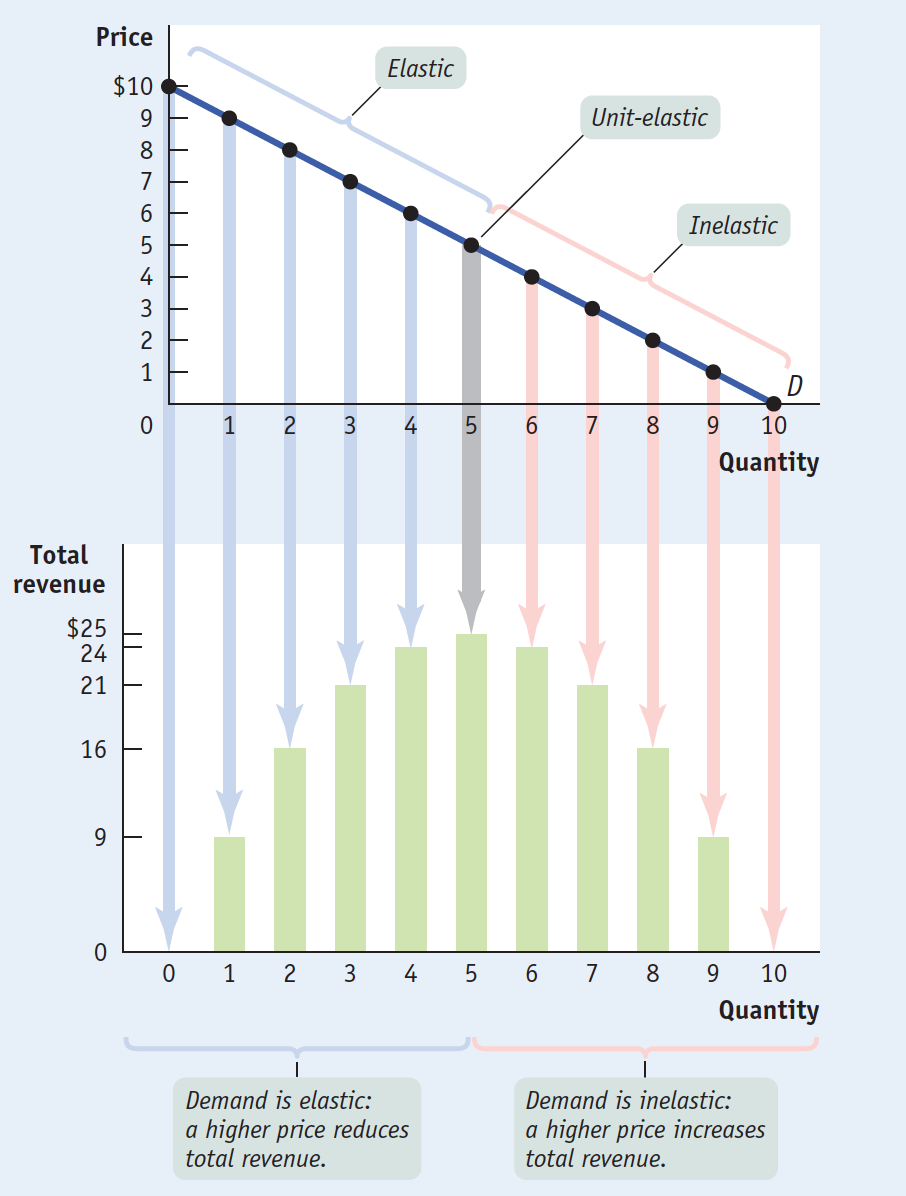
\includegraphics[height=0.8\linewidth, width=0.7\linewidth]{elasticVar}


\rem{The revenue maximum occurs when demand is unite-elastic}

\subsubsection{Factors of Influence}

\begin{enumerate}
	\item Luxury Vs Necessary Goods
	\par{Luxury goods tend to be much more elastic, since people can "live without them" which wither forces sellers to reduce the price or the quantity demanded is low}
	\item Availability of Close Substitutes
	\par{If there are close substitutes for a good, its price elasticity will be higher, again because people have choices}
	\item Share of Income Spent
	\par{ If people spend a large chunk of their income in a good, they don't mind spending time finding ways to reduce its quantity demanded, hence higher elasticity}
	\item Time Since Price Change
	\par{ Elasticity tends to increase with time}
\end{enumerate}

\subsection{Other Demand Elasticities}

\par{The quantity demanded of a good depends on variables other than price, we can study this variation with other elasticities}

\defn{Cross-Price}{measures the effect of the change in one good's price on another's quantity demanded

$$CP_{ab} =\% \frac{\Delta QD_{a}}{\Delta P_{b}}$$}

\rem{$a , b$ substitutes $\implies CP_{ab} > 0 \implies$ right shift of the D curve}

\defn{Income Elasticity}{measures the effect of a change in consumers' income on a good's demand
$$IED =\% \frac{\Delta QD}{\Delta I}$$}

\rem{Useful to understand if a good is inferior or normal}

\rem{If $IED > 0 \implies $ normal good}


\subsection{Price Elasticity of Supply}

\defn{Price Elasticity of Supply}{change in the quantity supplied in relation to a price change}

\subsubsection{Factors of Influence}

\begin{enumerate}
	\item Availability of Inputs
	\par{Elasticity tends to be large when inputs are readily available and can be shifted into and out of production at a relative low cost}
	\item Time
	\par{Elasticity grows larger as producers have more time to respond to price changes}
\end{enumerate}

\subsection{Elasticity Summary}
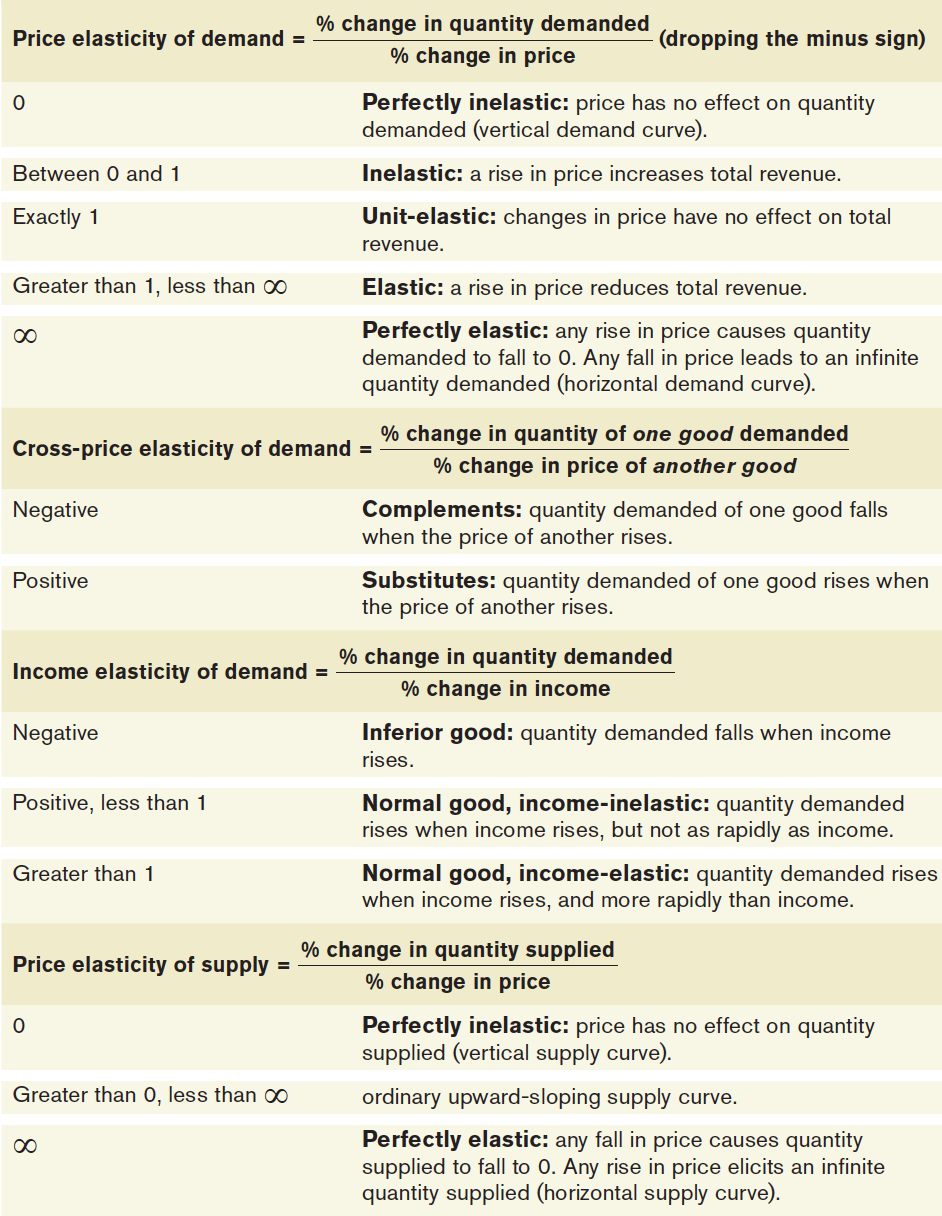
\includegraphics[height=1.1\textwidth]{elasticSum}
 
 \newpage
 
 \section{Taxes} 
\lecture{31}{01}{2019}

\defn{Excise Tax}{a tax charged on each unit of a good or service that is sold}

\par{Taxes have effects similar to those of quotas above. By imposing a tax on a good, the producer will tend to pass its costs onto the consumer. This will make goods in general more expensive, which in turn decreases demand.}
\par{So, \ita{for any given quantity} the amount producers are willing to charge is equal to that of Original Price + Tax. Which leads the supply curve to \ita{shift upwards by the tax amount}}

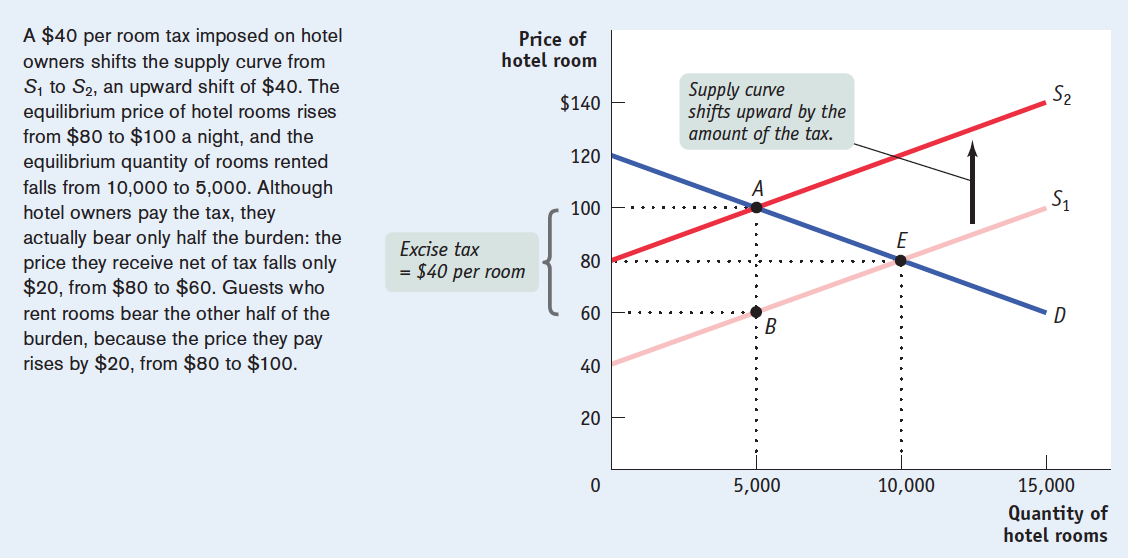
\includegraphics[width=\textwidth]{tax1}

\par{Note that in the example above, the consumers are paying 20\$ more than the original price, hence they are in effect paying half of the tax.}

\rem{Taxes can also be imposed on consumers, in which case the demand curve would be the one shifting. It would  of course shift downwards, since higher prices imply less demand}

\par{Note that regardless of who the tax is being imposed on, when looking at the same quantity (e.g. 5000), the guests pay in effect 100\$ and consumers 60\$}

\subsection{Incidence of a Tax}

\par{In the example above we've derived the \ita{general principle} that the outcome of taxation is the same regardless of who pays it. What is not necessarily true, is that the tax is always split 50-50. We can analyse the incidence of a tax by looking at price elasticity of supply and demand.}

\begin{itemize}
	\item[] Consumers: When the PED is low and the PES is high. This is because low PED $\implies$ few substitutes $\implies$ less flexibility. The reverse is true for supply, hence producers can use their "spare" goods for other purposes
	\item[] Producers: When the PED is low and the PED is high. This is because low PES $\implies$ few substitutes $\implies$ less flexibility. The reverse is true for demand, hence consumers can opt for similar goods.
\end{itemize}

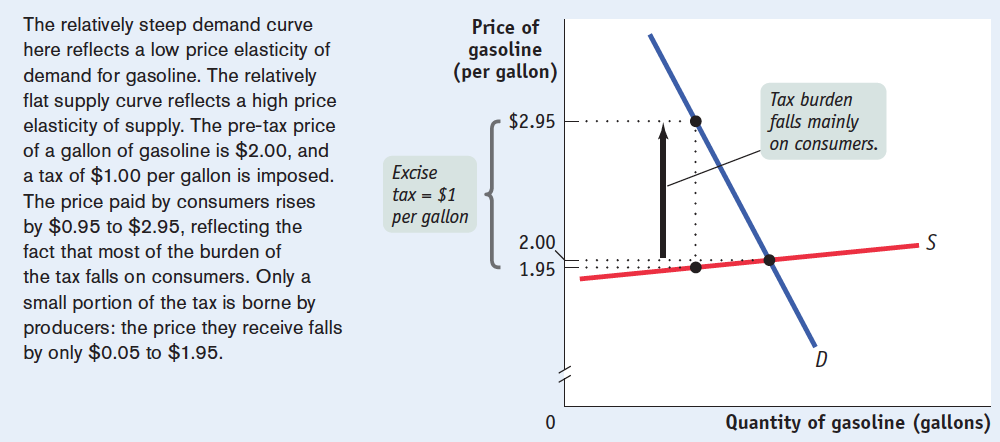
\includegraphics[width=\textwidth]{tax2} 
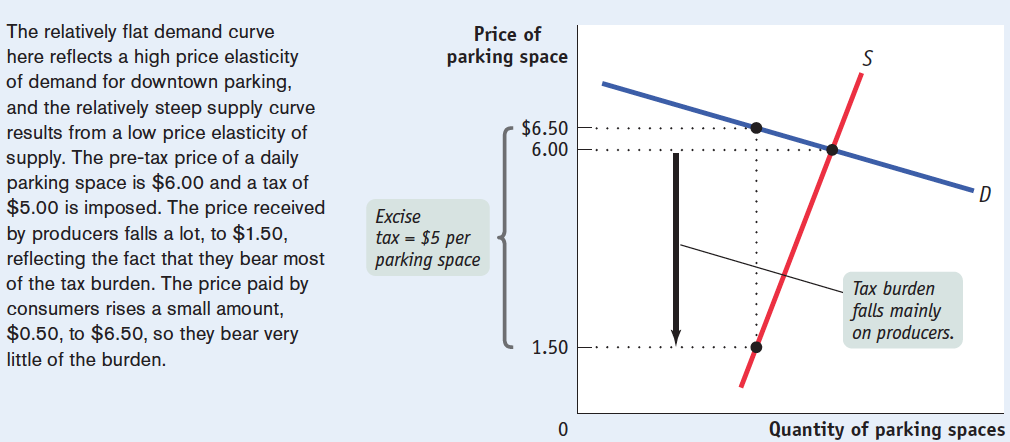
\includegraphics[width=\textwidth]{tax3} 

\subsection{Benefits and Costs of Taxation}

\par{The revenue collected from imposing a tax can be calculated by looking at the area of the triangle with height equal to the tax amount.\mymarginpar{look at quotas examples, for more a detailed analysis}. Once again, the net effect of raising a tax will depend on the elasticity of the curves.}

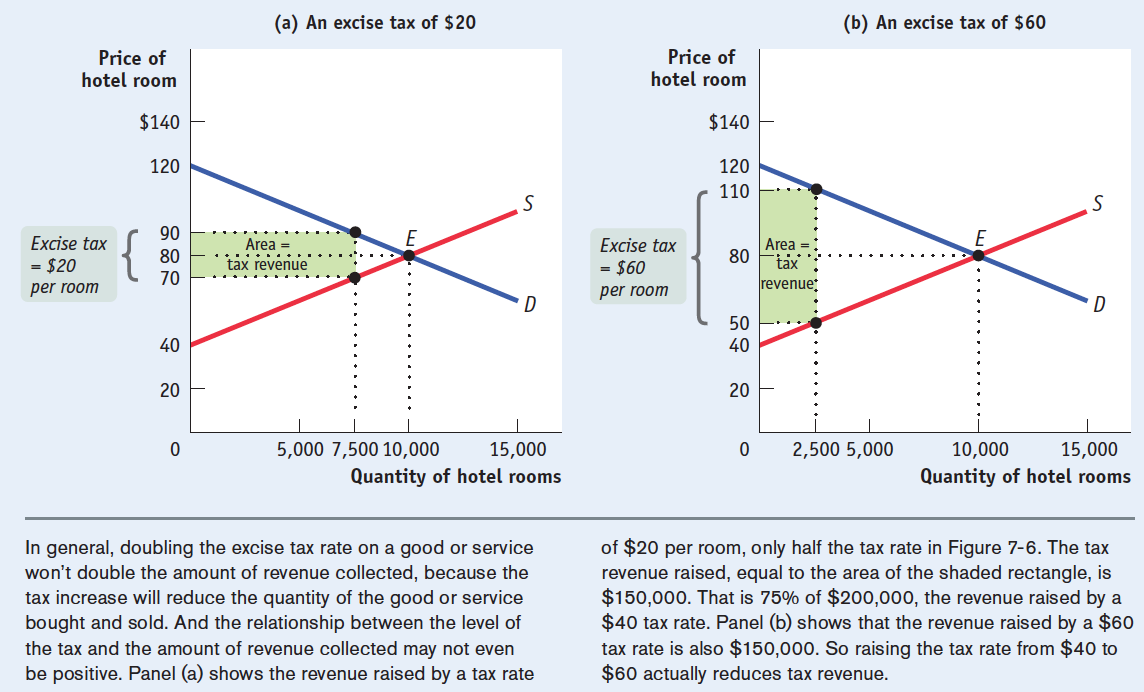
\includegraphics[width=\textwidth]{tax4}

\par{Given that the tax creates surplus, its costs are given by the \ita{deadweight loss} triangle}

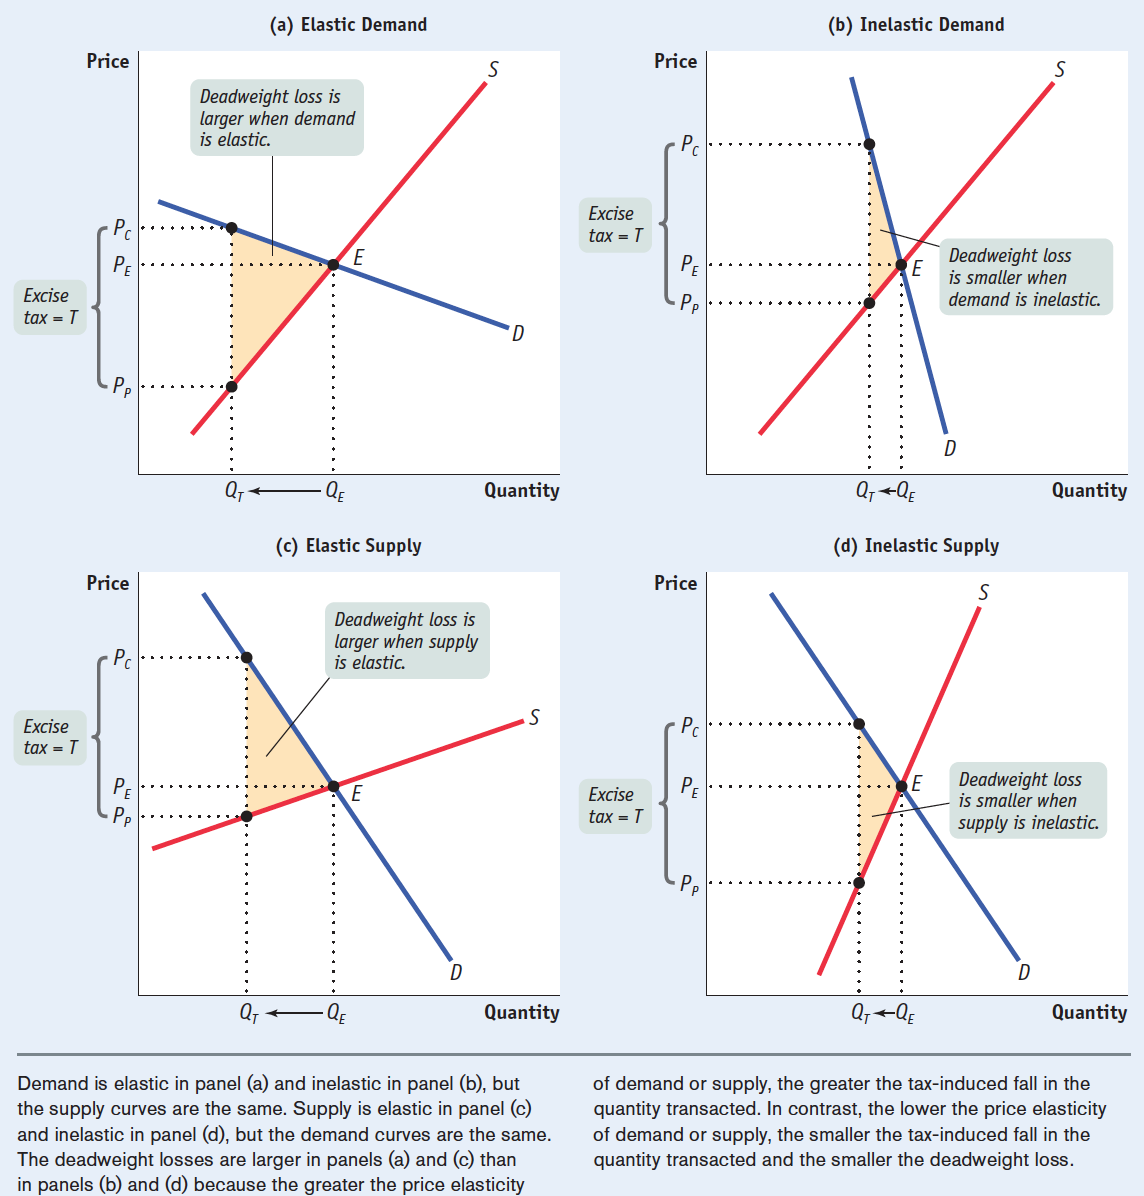
\includegraphics[scale=0.5]{tax5}

\section{Inputs and Costs}
\lecture{01}{02}{2019}

\subsection{Production Function}

\defn{Production Function}{Relation between the out/input quantities} 

\defn{Fixed Input}{Input whose quantity cannot vary in the \ita{short run}}

\defn{Variable Input}{Input whose quantity can vary depending on the firm's needs and wants}

\rem{Note that , in general, \ita{in the long run} all  inputs can vary}

\defn{Total Product Curve}{Graphic representation of the product function}

\par{The production function can be represented graphically for a given fixed input, where $x$ represent the var input and $y$ the output produced. We call this curve the \ita{total product curve}. Note that from this representation one quickly obtains useful info : \ita{e.g} positive slope $\rightarrow$ increased output with increase of input}

\defn{Marginal Product}{The additional quantity of output that is produced by increasing input by 1 unit, i.e. the ratio between change of output and input. Example: Marginal Product of Labor (where labor is the var input)}
$$MP = \frac{\delta Q}{\delta L}$$

\par{We say that a firm enjoys increasing \ita{returns to scale} or \ita{marginal product}, if the amount of input needed to produce one more unit is less than what was needed to produce the unit before it (and vice-versa). Mathematically speaking, the curve will have a negative slop, since $\delta Q < 0$}  

\rem{When calculating, remember to be consistent with units. For example, it would be wrong to compare the output added by an additional hour of labor with the cost of employing a worker for a week}

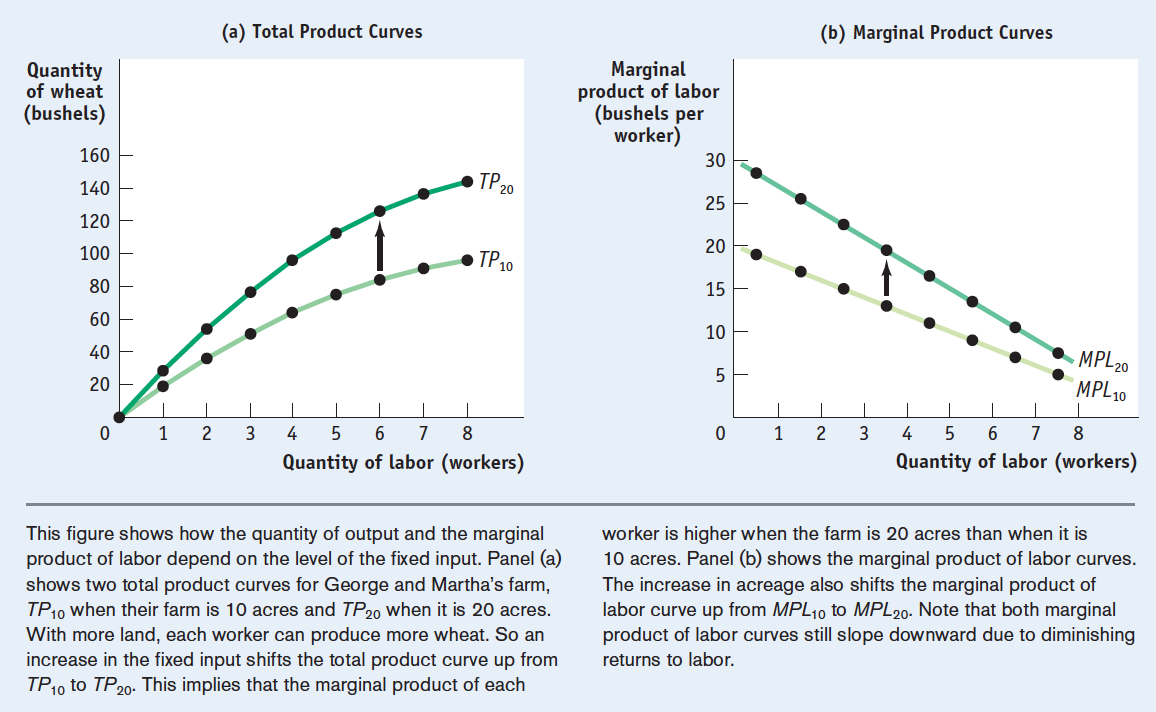
\includegraphics[width=\textwidth]{totalMargProduct}

\subsection{Total Costs}
\lecture{05}{02}{2019}

\par{We can translate our production function onto a \ita{cost curve}, which relates output with cost. We represent the output in the $x$ axis and total cost in the $y$ axis.}

\defn{Total Cost}{Is the sum of the costs of the fixed inputs, and variable inputs}
$$TC = FC + VC$$

\rem{FC is invariant with output, hence : FC = TC, for $0$ output} 
\par{ Again it should be intuitively obvious, that the curves will vary inversely, since to say that input A shows 'diminish returns' is the same as saying that ''after a certain point , increasing input comparatively produces less input'' which in terms of profits/costs is the same as saying that ''after a certain point, increasing input costs more'' hence, increased output will lead to costlier variable costs (inputs), which will lead to higher TC}

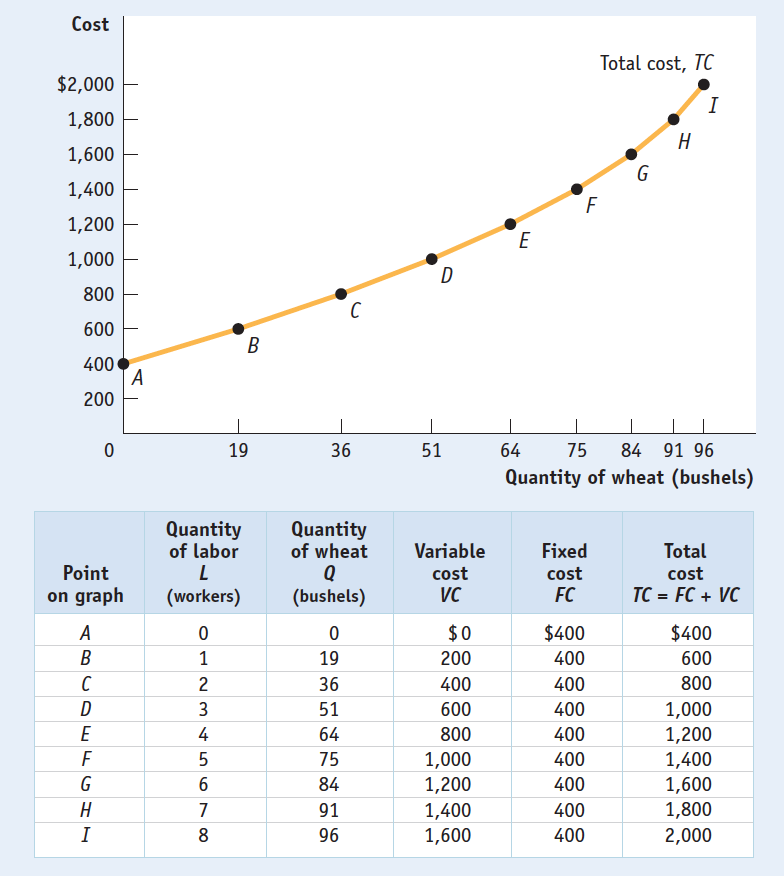
\includegraphics[height=0.5\textwidth]{totalCost}

\subsection{Marginal and Average Cost}

\defn{Marginal Cost}{Change in total cost generated by producing one more unit of input}

$$MC = \frac{\delta TC}{\delta Q}$$

\rem{By the paragraph above, one expects the MC curve to be proportional to that of cost}

\defn{Average Total Cost}{Total cost \ita{per unit} produced}

$$AC = \frac{TC}{Q}$$

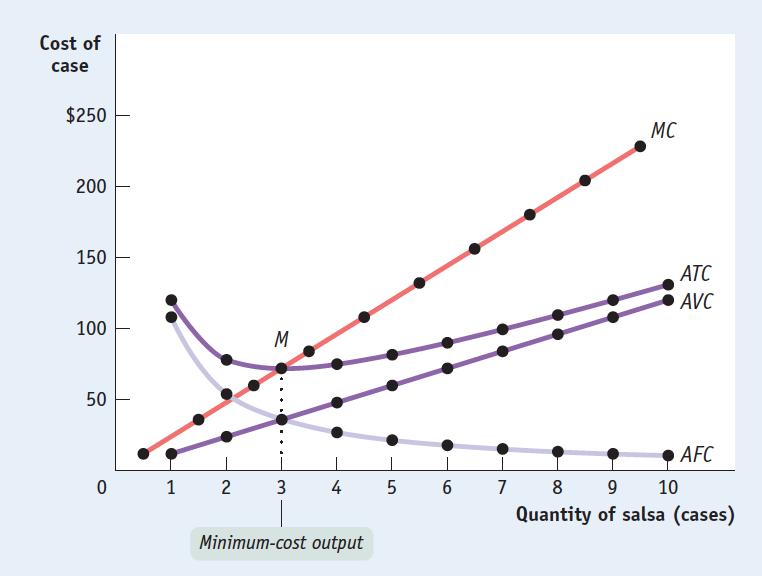
\includegraphics[width=\textwidth]{avgCost}

\par{Much like TC, we can break AC into its component parts, that of fixed and variable costs. We can then see that for small outputs, fixed costs would be relatively high, but will in turn decrease, since the output quantity will not affect its costs (key: they're fixed). So, the cost of the fixed input will be \ita{spread} around the units produced (e.g. same land, more vegetables, less costly).}
\par{On the other hand, the costs for variable inputs start small but grow with the growth of the input (key: they're variable). And in the case of diminishing returns, the effect of this cost will eventually overcome the \ita{spreading effect} (e.g. more workers, eventual productivity plateau, higher salary costs)}
\par{Hence, AC has this unique U shape, exemplifying the inverse relation between AFC and AVC}

\par{In sum: increasing output has two opposing effects on AC:}

\defn{Spreading Effect}{ The larger the output, the greater the quantity of output
over which \ita{fixed cost is spread}, leading to lower average fixed cost.}
\defn{Diminishing Returns Effect}{The larger the output, the \ita{greater the amount of variable input required} to produce additional units, leading to higher average variable cost.}

\defn{Minimum-Cost Output}{The quantity of output that corresponds to the minimum AC}

\par{Obviously we should expect profits to be maximum, when average cost is minimum. We can compare this with the optimal quantity of our demand curve. Hence 3 principles can be derived from MC and AC relation:}

\begin{enumerate}
\item At the minimum-cost output \textbf{MC = AC} 
\item Below minimum-cost, AC is falling (room to increase output at a profit)
\item Above minimum-cost, AC is increasing (not worth increasing output)
\end{enumerate}

\par{These are easy to derive, if we think in terms of averages. Given that if MC is below AC, then that means that there is still room to increase output, i.e. the cost of producing one unit (MC) is still \ita{lower} than the average cost per unit produced, and so it will lower AC}

\rem{In real-life, at low levels of output there are often increasing returns to the variable input due to the benefits of specialization, making the marginal cost curve U shaped also}


\subsection{Short and Long Run}
\lecture{07}{02}{2019}

\par{In the long-run FC is no longer fixed, we have then a \ita{family} of short-run ATC. Changes in output will lead to moves along a specific short-run ATC curve, but if a firm finds that change to be long-term, it will most likely find another curve which suits its needs better, i.e. it will want to adjust its fixed cost in order to minimize ATC, effectively moving to a different short-run curve}

\defn{Long-Run Average Total Cost Curve}{The relationship between output and average total cost when fixed cost has been chosen to minimize average total cost for each level of output}

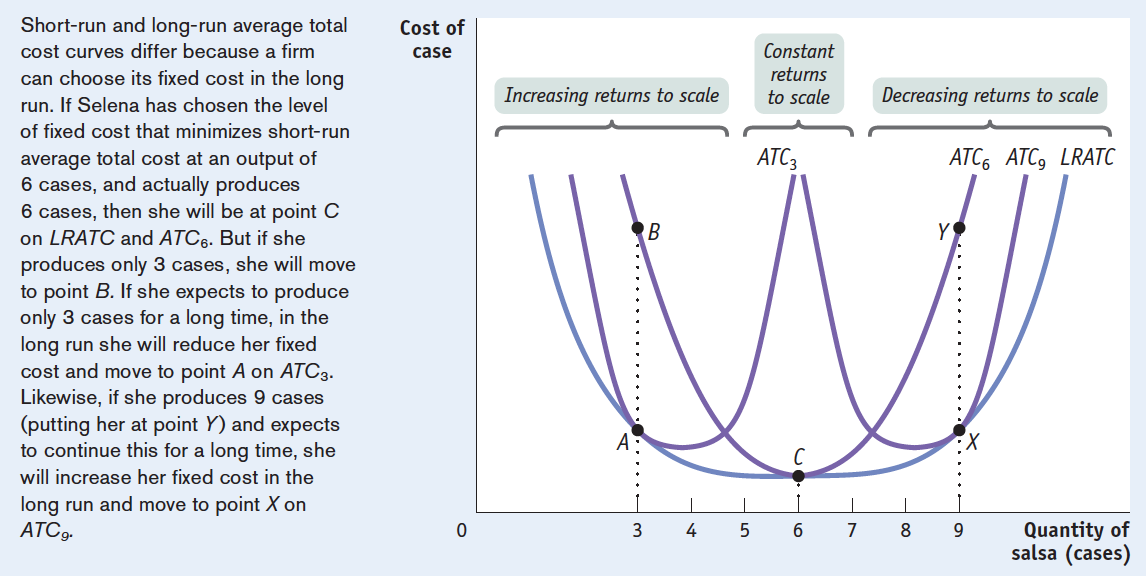
\includegraphics[width=\textwidth]{LRATC}

\par{Crucial to understanding when to move is to decide if the company size needs to grow or if the increase in output is an aberration. For example, say a firm supplies car parts, on average one small size warehouse is enough, apart from every other winter where extra space is rented from 3rd party. However, a year later, after a couple new contracts, the quantity of constant output increases to peak numbers. To rent the other space is no longer sustainable, hence, the firm will most likely decide to buy a bigger warehouse, which can accommodate all its stock. In the \ita{long-run} this will bring ATC down, i.e there will be \textbf{increasing returns to scale}}

\defn{Scale}{Size of a firm's operations}

\defn{Returns to Scale}{Increasing when \ita{long-run} ATC decreases as output increases (and vice-versa)}

\begin{itemize}
	\item[] Causes of Increasing RS
	\begin{enumerate}
		\item Increased Specialization: individual workers are more efficient at specific tasks
		\item Very large initial setup cost, e.g. construction power plant
		\item Network Externalities: the value of a service to an individual increases when a large number of others own or use the same good or service
	\end{enumerate}
\end{itemize}


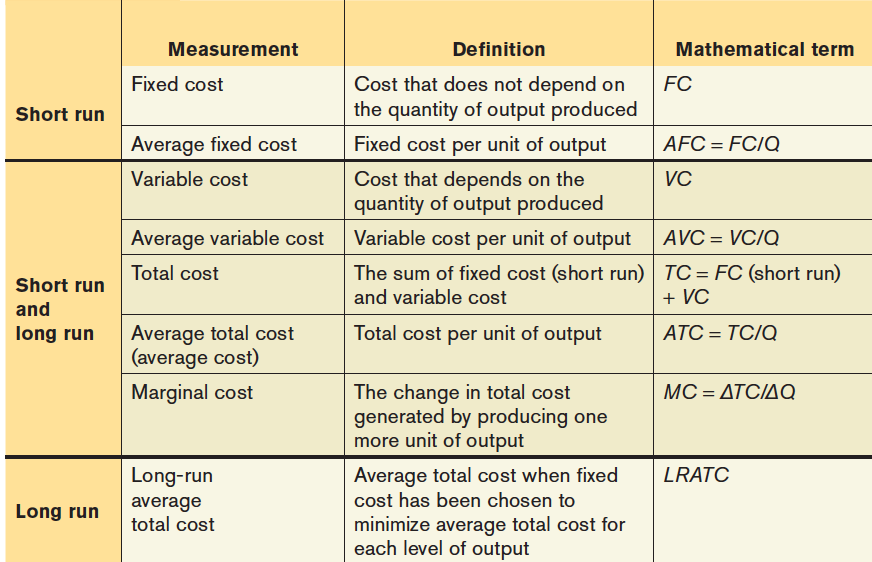
\includegraphics[width=\textwidth]{SummaryCosts}


\newpage

\section{Perfect Competition}
\lecture{07}{02}{19}

\defn{Price-Taking
Producer/Consumer}{A producer/consumer whose actions have no effect on the market price of the good or service it sells.}

\defn{Perfectly Competitive Market}{Market in which all market participants are price-takers.}

\defn{Perfectly Competitive Industry is an industry in which producers are price-takers}

\rem{The supply and demand model, is a model of a perfectly competitive market. It
depends fundamentally on the assumption that no individual buyer or seller believes that it is possible to affect
the price at which he or she can buy or sell the good.}

\subsection{Necessary Conditions for Perfect Competition}

\defn{Market Share}{Fraction of total output accounted for by a certain producer's output}

\defn{Standardized Output / Commodity}{When consumers regard products from different producers as the same good}

\begin{enumerate}
	\item It must contain many producers, none of which may have a large \ita{market share}
	
	\item The industry output must be a standardized good
	
	\item Free Entry \& Exit : There must not be any regulations or limited access to key resources, that prevent firms from entering and leaving the market
	
\end{enumerate}

\example{ Wheat Vs Cereal Flakes
\par{(1) Many producers, none has significant market share Vs Handful of brands}
\par{(2) Standard Commodity, wheat is all the same. Increasing price will lead buyers to go elsewhere (Perfect Substitute). Vs Many different type of cereals, increasing Raisin Bran will not affect Kellog's Special K sales}
}

\subsection{Production \& Profits}

\defn{Marginal Revenue}{Change in total revenue generated by an additional unit of output}

$$MR = \frac{\delta TR*}{\delta Q}$$ \mymarginpar{*Total Revenue = Quantity $\times$ Price}

\defn{Profit-Maximizing Principle}{The optimal amount of an activity is equal to the lower bound MC = MR, i.e. the maximum quantity possible up to to the point where MC = MR}

$$\boxed{MR = MC}$$

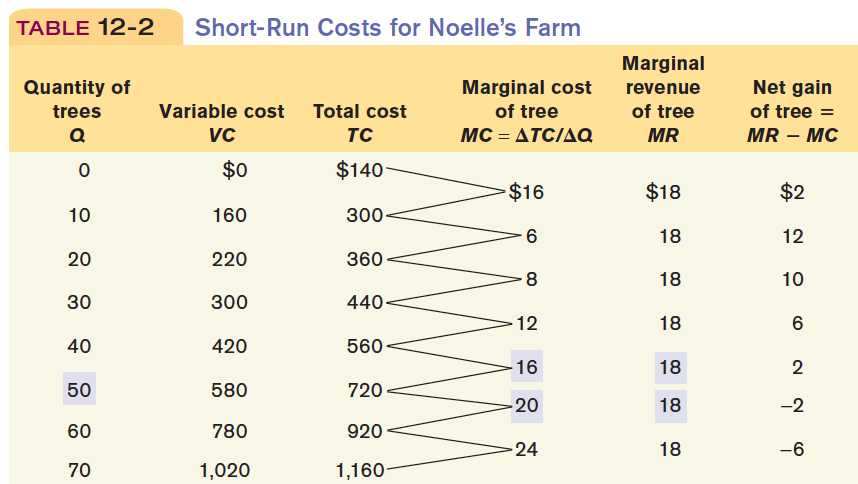
\includegraphics[width=0.6\textwidth]{OptOutput}


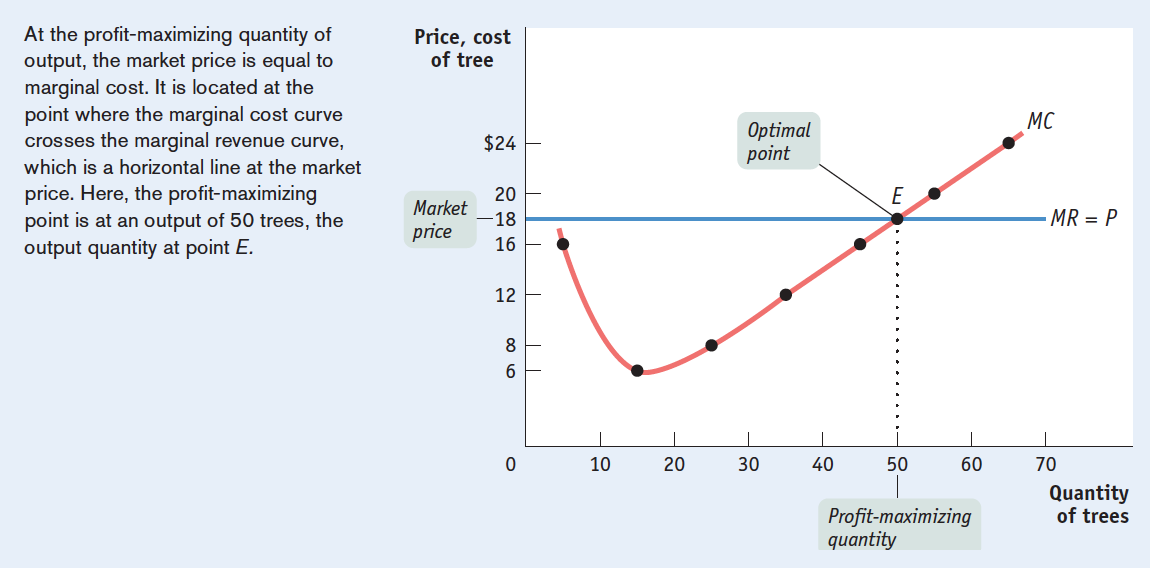
\includegraphics[width=\textwidth]{optimalPrice}

\par{The graph above exemplifies a restatement of the principle above}

\rm{In a competitive market MR = Market Price}

\defn{Price-Taking Firm's Optimal Output Rule }{A price-taking
firm's profit is maximized by producing the quantity of output at which the market price is equal to the marginal cost of the last unit produced. $P = MC$}

\subsubsection{Profitability}

\par{Remember that  : Profit = Total Revenue - Total Cost. Hence, it clearly follows that a firm is profitable if:}

\begin{itemize}
	\item TR $>$ TC : Profitable
	\item TR $=$ TC : Break-Even
	\item TR $<$ TC : Unprofitable
\end{itemize}

\par{Instead of looking at the totals, we can express the idea above by using the concept introduced before of total averages, i.e. where we look at the revenue and cost per unit of output}

$$\frac{1}{Q} \times P = \frac{1}{Q} \times (TR - TC)$$

\par{Note, however that as seen before, $\frac{TC}{Q} = ATC$ and $\frac{TR}{Q}$ is the average revenue (Market Price), hence simplifying the equation above we conclude that a firm is profitable if \ita{its market price is higher than its average total cost}

\begin{itemize}
	\item P $>$ ATC : Profitable
	\item P $=$ ATC : Break-Even
	\item P $<$ ATC : Unprofitable
\end{itemize}


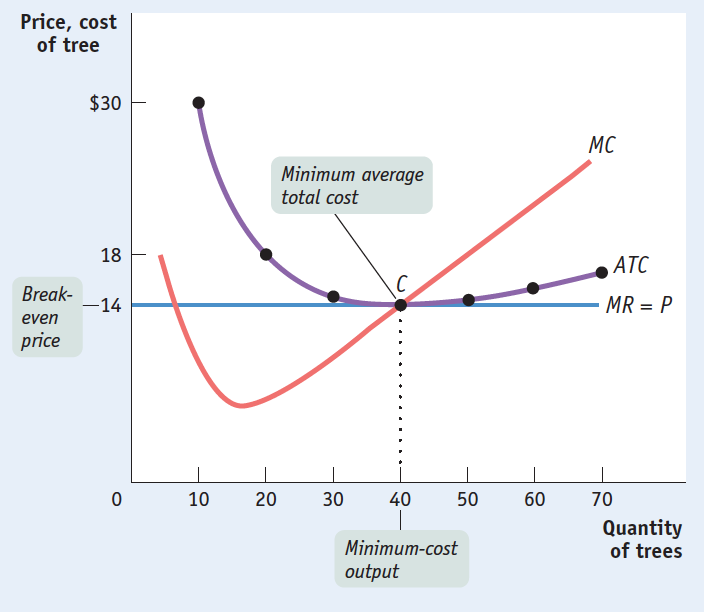
\includegraphics[width=0.7\textwidth]{profit}


\rem{Note that MR and MC are not a direct indication of profitability, since a firm can be profitable in the whole (TR $>$TC) whilst having a MR $<$ MC, which just indicates that the firm can become even more profitable by improving its revenue margin, i.e. by cutting costs}

\newpage
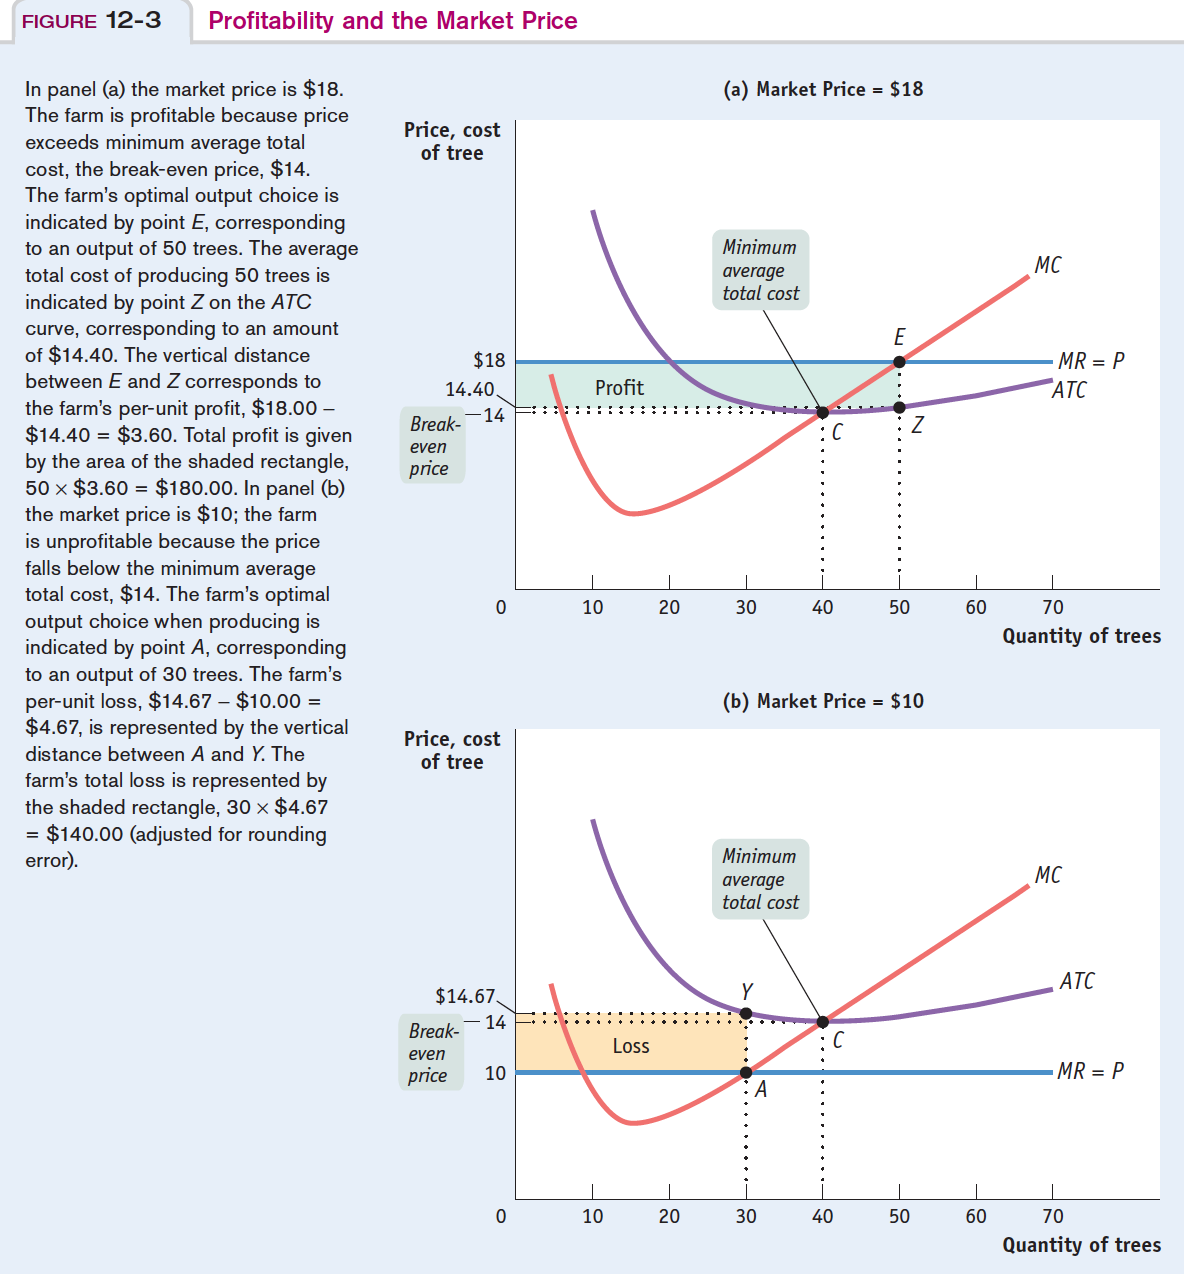
\includegraphics[width=\textwidth]{profit2}

\newpage
\subsection{Production Decision}

\par{Sometimes just because a firm is unprofitable \ita{in the short run}, it doesn't mean that it should halt production, since it will still have to cover its fixed costs. On whether to decide when to stop, a firm must look at its variable costs}

\par{In particular, we need to compare market price with the firm's AVC. If, }

\begin{itemize}
	\item P $<$ AVC : this means that the firms is not covering its costs at all at any point, i.e. not only is the firm incurring a necessary loss from its fixed costs, but is also incurring total losses for producing those new units. Hence, it should halt production. Maximising profits by minimising losses to those of the FC only. 
	$$\text{Shut-Down Price = Minimum Average Variable Cost}$$
	\item P $>$ AVC : the firm maximizes profits/minimizes losses by choosing the output quantity at which its marginal cost is equal to the market price.
\end{itemize}

\defn{Shut-Down Price}{the price at which the firm shuts production in the short run}

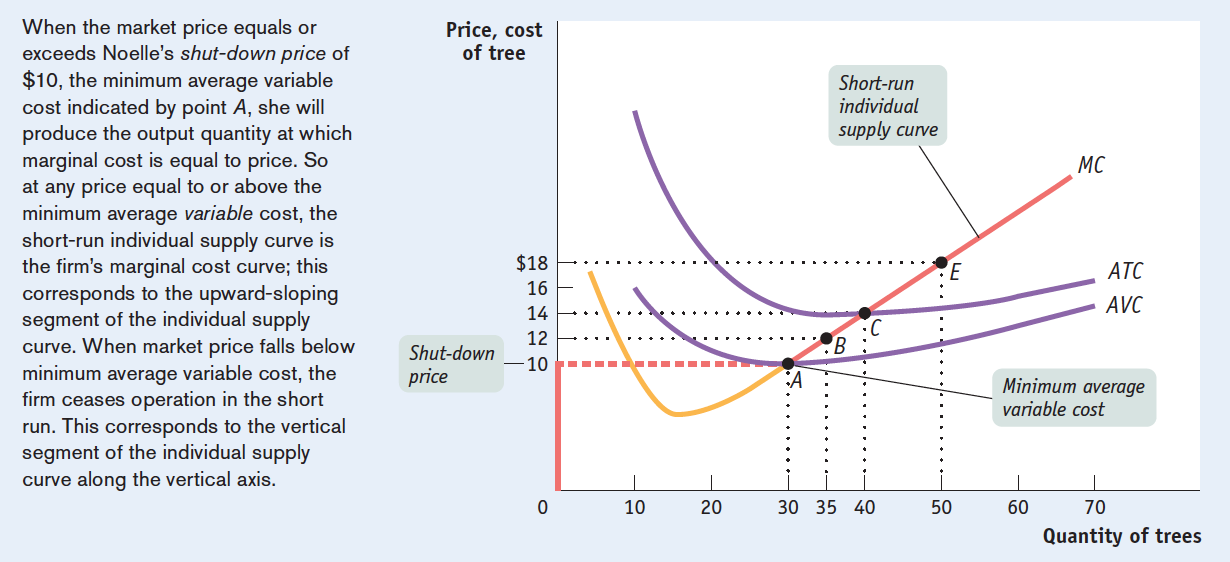
\includegraphics[width=\textwidth]{profit3}
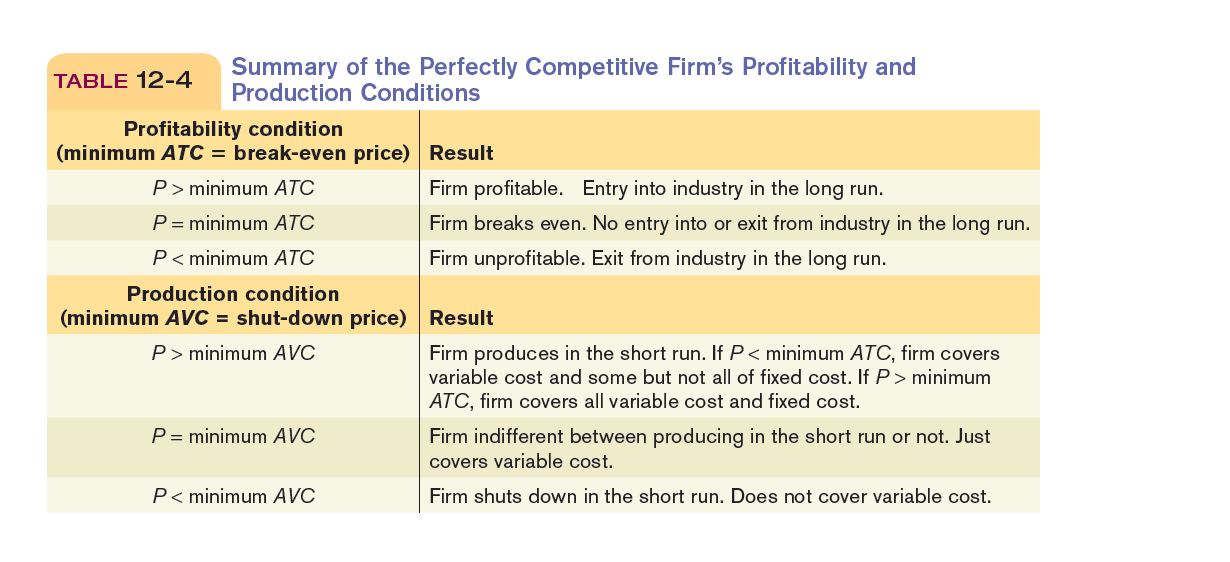
\includegraphics[width=\textwidth]{profitSum}

\newpage

\subsection{Industry Supply Curve}

\defn{ISC}{Relationship between the price and the total output of an industry as a whole}

\subsubsection{Short-Run Vs Long-Run}

\par{In the short-run the number of producers in an industry is fixed, there is no entry or exit. Hence, its supply curve will depend only on the quantity that producers will supply at any given price, but taking the number of producers as fixed}

\par{On the other hand, in the long-run the numbers of producers often varies. Producers seeing that an industry is profitable will want to join it, which in turn will cause the supply curve of the industry (aggregate of the individual firms' supply) to shift to the right, and will lead to the lowering of the equilibrium price.}
\par{How do existing firms react? They will lower production, in order to cut variable costs. This will happen until a final equilibrium is reached, where it is no longer profitable for new firms to join, or existing ones to exit - \ita{long-run market equilibrium}. Which as previously seen, happens at the point of break-even (minimum ATC)} }

\rem{remember that when saying that break-even = zero \textbf{economic profit} means that the industry is performing at market average. Obviously they still have net profits, but the market is now saturated, the large initial gains (e.g. startups) are gone and now gains are shared amongst competitors}

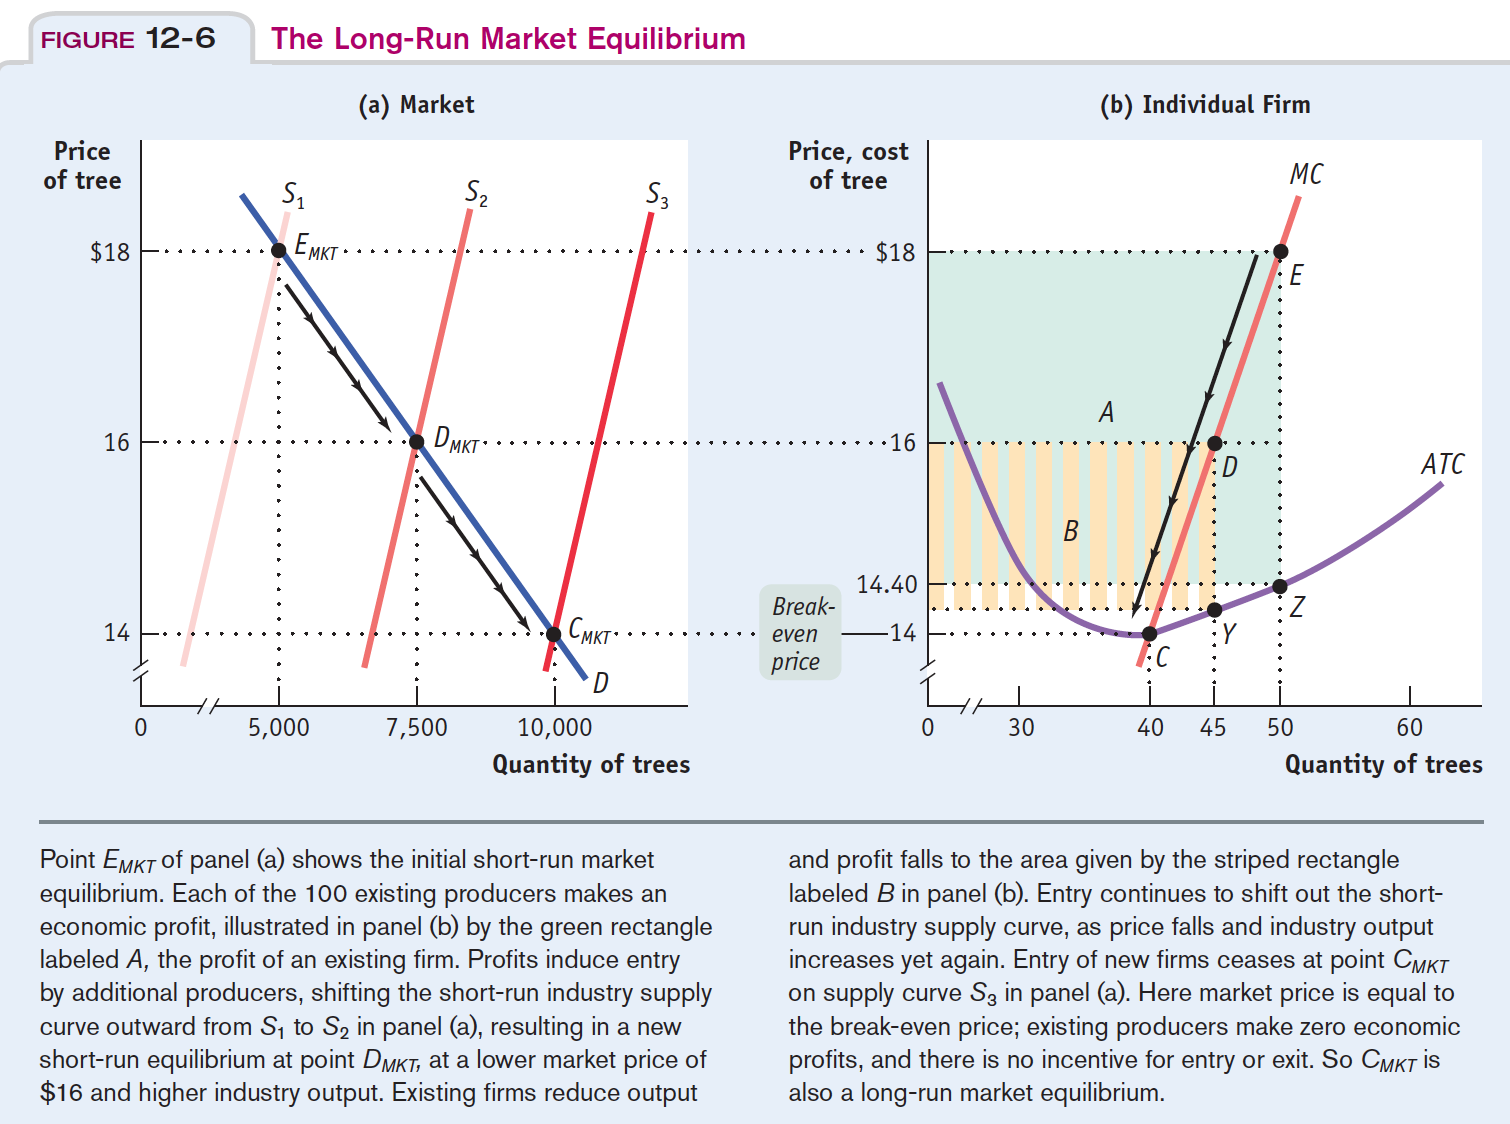
\includegraphics[width=\textwidth]{longRunEntry}

\subsection{The Cost of Production and Efficiency in Long-Run Equilibrium}

\par{Hence, to summarize, in the long-run:}

\begin{enumerate}
	\item The Value of MC is the same for all firms: given that the price is the same for all firms (MP = MC), every firm will want to maximise profits (we assume that firms are operating as optimal rational agents)
	\item Each firm will have zero \ita{economic} profit: The money will flow towards the industries that are performing better, until eventually it becomes saturated
	\item No mutually beneficial transactions will go unexplored (Efficient)
\end{enumerate}

\section{Monopoly}

\subsection{Market Structure}

\par{There are many different types of markets, divided into 4 principal models (perfect competition, monopoly, oligopoly, and monopolistic competition) in accordance to 2 main criteria }

\begin{enumerate}
	\item Number of producers in the market
	\item Whether the goods are standardized or differentiated 
\end{enumerate}

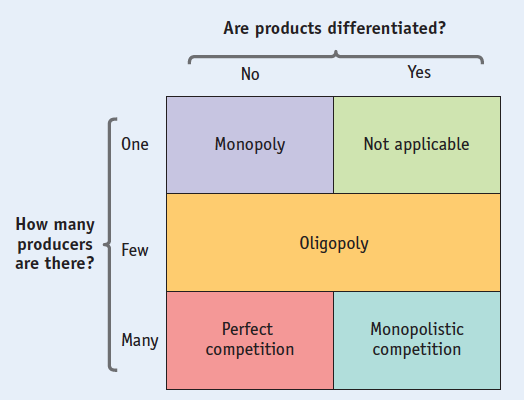
\includegraphics[width=0.5\textwidth]{marketStrut}

\defn{Monopoly}{Industry controlled by a monopolist}

\defn{Monopolist}{A firm that is the only producer of a good with no close substitutes}

\defn{Market Power}{The ability of a monopolist to raise prices above the competitive level by reducing output}

\par{Unlike in the competitive model, monopolists are able to affect market prices by reducing quantity supplied. Since there are no close substitutes, consumers are bound to buy their products. Less Supply $\rightarrow$ Less Costs + Higher Price $\rightarrow$ Higher Profits}

\subsection{Barriers to Entry}

\par{Given that the monopolist is operating at above zero economic profit, why don't other firms entry the market?}

\begin{enumerate}
	\item Control of a Scarce Resource 
	\item Increasing Returns to Scale : Initial players are able to spread high fixed costs, in particular due to existing number of customers and high initial gains. In an industry with IRS, ATC will keep plummeting, allowing firms to grow larger and larger, whilst making the costs of entry prohibitively expensive for new companies. This leads to the emergence of \ita{natural monopolies}
	\item Technological Superiority (short-run)
	\item Network Externalities
	\item Government Imposed Barriers : patents and copyrights
\end{enumerate}

\subsection{Maximising Profits}

\par{Because a monopolist has absolute control over supply, its demand curve will be equal to that of the market. For example, in a competitive market moving away fro market price, will immediately mean that quantity demanded falls to $0$, since people will look elsewhere (demand curve is horizontal). On the other hand, monopolists can move along the demand curve, since increasing demand will increase revenue per unit (at which that new unit is sold) - \ita{quantity effect} , i.e. more people will buy their goods. But will also cause TR to come down (each unit is cheaper) - \ita{price effect} . The point at which the price effect is minimum, and the quantity effect is maximum is the profit maximising point}

$$\boxed{MR = MC}$$

\rem{Revisit elasticity for a similar discussion}

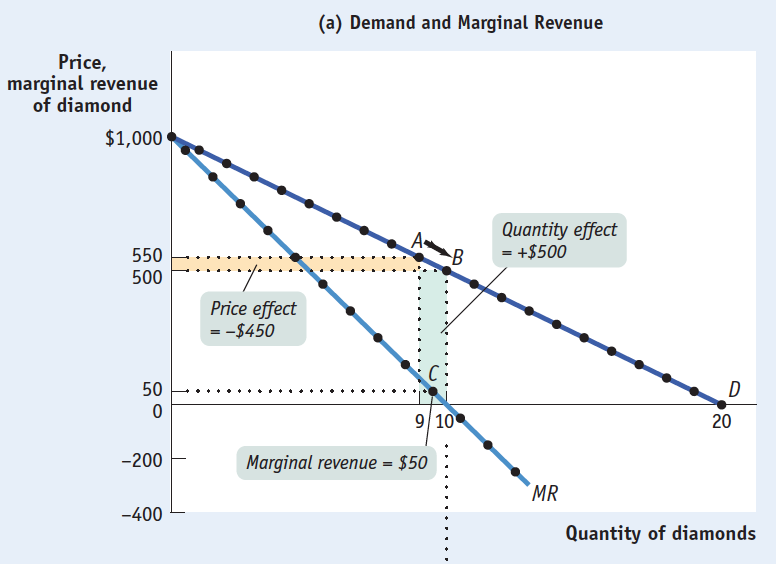
\includegraphics[width=0.5\textwidth, height=0.5\textwidth]{mon}
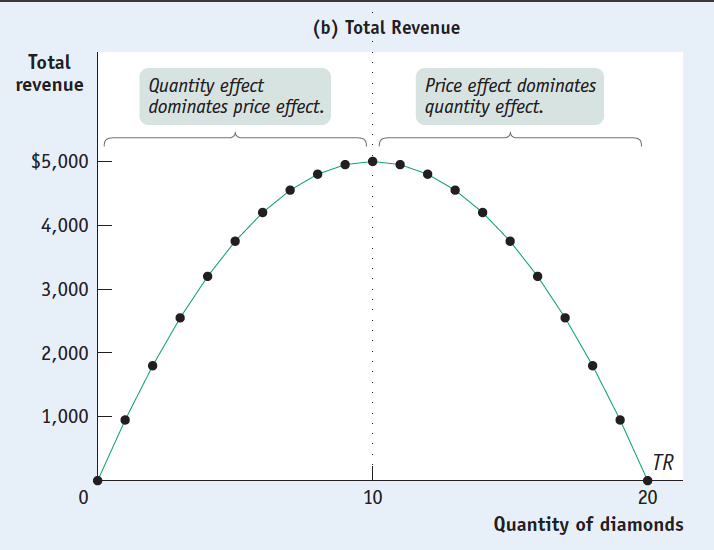
\includegraphics[width=0.5\textwidth, height=0.5\textwidth]{mon2}

\par{Looking more generally at what happens in the monopoly, using marginal analysis we have the following}

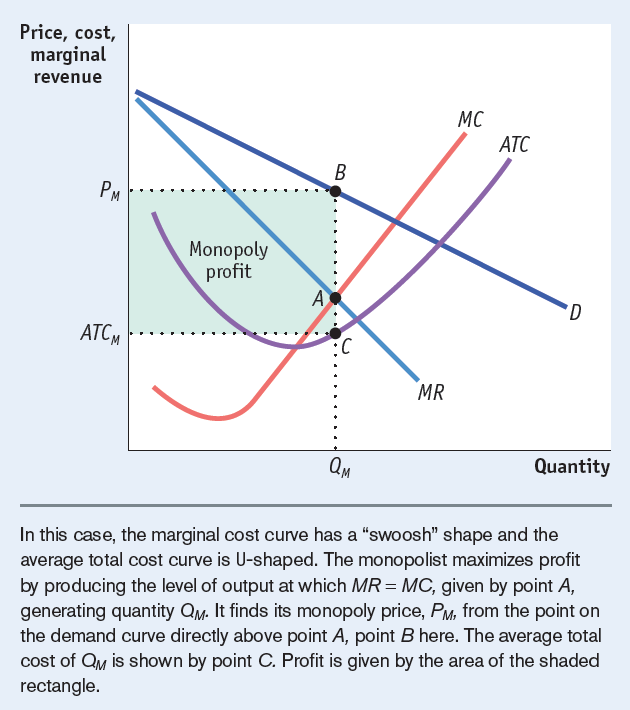
\includegraphics[width=0.5\textwidth, height=0.5\textwidth]{mon3}

\par{Remember that profit is equal to revenue - costs. We know from the optimal output rule that the optimal price happens when MR = MC, and so looking at the demand curve, we can see that $TR = P_{M} \times Q_{M}$ . Now, looking at the average costs curve $TC = ATC_{M} \times Q_{M}$. Subtracting both, we have the maximum profit given by the green rectangle}

\subsection{Inefficiency and Public Policy}

\par{Producers do much better in a monopoly than in a competitive market, since as we've seen they operate above the zero economic profit. But where do these gains come from?}
\par{In essence, a monopolist by moving up the demand curve decreases consumer surplus, and increases producer surplus which it turns to profits. However, when looking at Total Surplus, we find that it is less than in the competitive market, necessarily meaning that it creates losses for society - deadweight loss. (There are many consumers willing to trade, which are being prevented due to the high prices)}

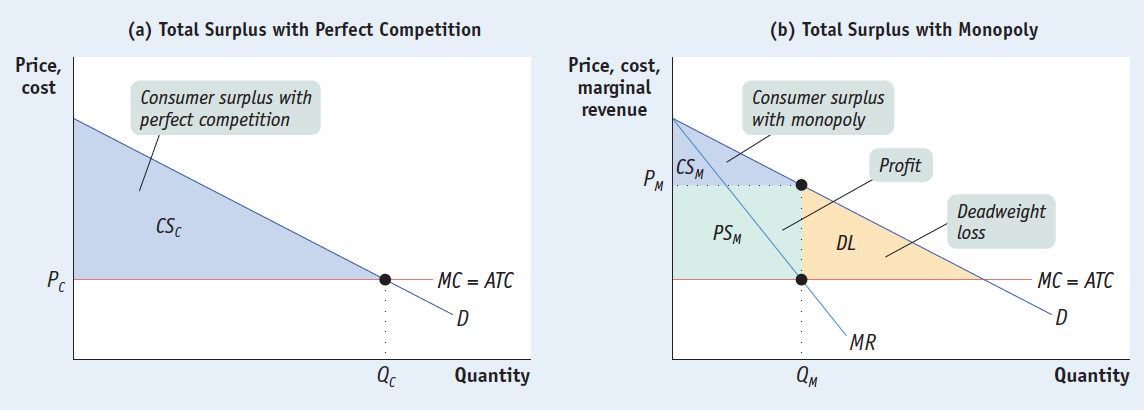
\includegraphics[width=\textwidth]{mon4}

\par{This leads governments and policy makers to want to avoid the emergence of monopolies. In general policies like antitrust laws were enough to prevent this, but as we've just seen, it often happens that \ita{natural monopolies} emerge, where natural barriers prevent competitors from entering the market, as opposed to other firms.}
\par{In is often unclear whether a natural monopoly will create losses for consumers if broken (e.g. higher prices energy sector), however they still cause inefficiency, since prices above market average will prevent transactions. Governments can intervene in two major ways}

\begin{enumerate}
	\item Public Ownership : If an industry is seen to be as a possible (or even actual) natural monopoly, then the government creates a publicly owned firm to run it. In this way, consumers interests are put above profits. There is an argument against this route, given that public entities are not profit-motivated they are less prone to want to cut costs or improve services \mymarginpar{Why would monopolies want to improve services though? }
	\item Regulation : Limit prices
\end{enumerate}

\section{Oligopoly}

\defn{Oligopoly}{An industry with only a small number of producers}

\par{Oligopoly is a type of industry where no a single producer can affect market prices, but the model is still marked by imperfect competition, since a handful of players can. Up until this point, to determine how much output a firm would produce, we needed to look at the quantity that maximised profit. However, things are not as straightforward in oligopolies.}

\defn{Duopoly}{Oligopoly consisting of only 2 firms}

\defn{Collusion}{When firms cooperate to raise their joint profits}

\defn{Cartel}{An agreement among several producers to obey output restrictions in order to increase their joint profits (e.g. OPEC)}

\par{In this case, the firms would quickly realize that by engaging in intense competing with each other, each trying to outdo the other by producing more and driving down prices, they would eventually reach the stage of zero economic profit. Surely, with so much profits available to be made, they would want to avoid that. One way this can be done is by \ita{colluding} with each other. By agreeing on a max output, they make sure that TR doesn't fall behind a certain agreed threshold. }

\subsection{Competition}

\par{Having set a max output quantity, a dishonest firm will have big incentives to cheat. Since it would be able to drive its prices down, whilst having more units to sell than its competitor}

\par{For example, if the 2 companies agree to sell a max of $20$ units at a price of $10$\pounds \ , then their individual total revenue would equal $200$\pounds. Note however, that if one of the firms manages to drive prices down to $9$\pounds, then it would make an extra $9$\pounds \ for every unit it sells above the agreed max output quantity.}

\par{So, even though both companies would in the long run be better off by cooperating the uncertainty as to how the other firm will behave makes it difficult to predict output (e.g. prisoner's dilemma) }

\subsubsection{Game Theory}

\par{One way to analyse and decide on how to act when firms' actions are inherently interdependent is by resorting to game theory \mymarginpar{decision 2 notes}}

\defn{Pay-Off Matrix:}{the pay-off for each combination of strategies, seen from a player's POV, can be represented in matrix form.}


\defn{Dominant Strategy}{best action regardless of other player's one, i.e. best worst-case scenario (maximin)}

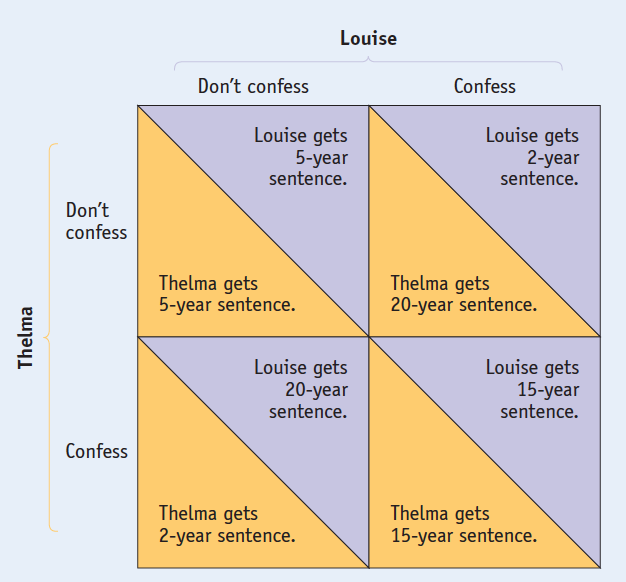
\includegraphics[width=0.5\textwidth]{g}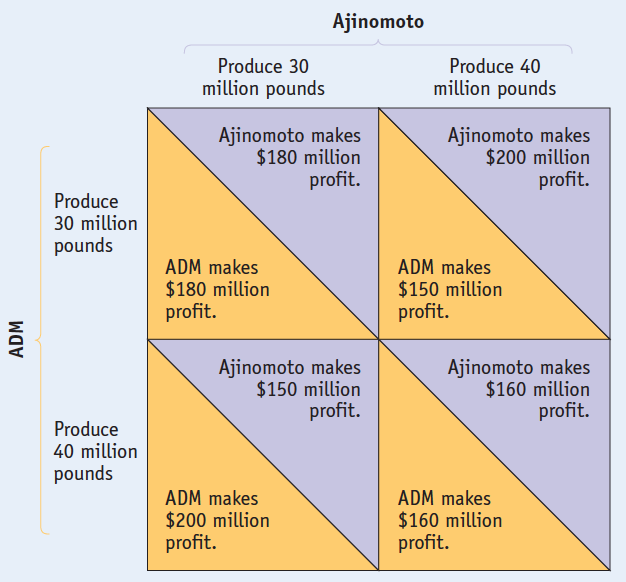
\includegraphics[width=0.5\textwidth]{g2}

\par{So, in the first example and taking prison years to be negative:}
\par{Min(C) = -15 and Min(NC) = -20 hence, choosing the best possible scenario is Max(-15,-20) = -15. Hence, regardless of what the other does, they're both always better off confessing}
\par{Similarly, in the second example, both firms want to avoid dropping their profits to $160\pounds$, so its best if they choose $30$} 

\defn{Nash Equilibrium}{each firm chooses the action that maximizes its payoff given the actions of other players, ignoring the effects of its action on the payoffs received by those other players, i.e. we want minimize losses, maximin}

\par{In oligopolies, firms do not play \ita{one-shot} games, instead they play repeatedly and against the same players, this implies that their actions will have consequences on other firms' future actions. In order to maximise gains they must engage in strategic behaviour, attempting to influence the future behaviour of other firms.}
\par{As we've seen, if a firm cheats it might incur temporary gains, but in the next round the other firm will match its production, and in the long-run both companies will lose profits. The awareness of this fact means that even without formal agreements, most oligopolies will function around \ita{tacit collusion}}


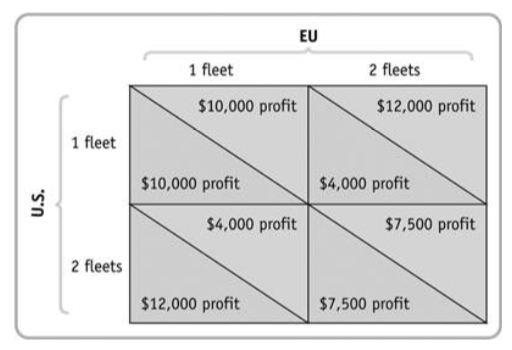
\includegraphics[width=\textwidth]{g3}

\par{Compare cooperative vs non-cooperative nash-equilibrium in the pay-off matrix above.}
\par{In a one-shot game, the firms will want to choose their best worse-case scenario, hence as explored above they will both choose to send 2 fleets, even though they are forfeiting $2.5$K from cooperating}
\par{Afterwards, by being aware of the lost profits and of each other's strategies, they will employ a tit-for-tat strategy, and send only one boat}


\section{Monopolistic Competition}
\mymarginpar{Not covered}
\par{Characterized by}

\begin{enumerate}
	\item Large numbers of competing producers
	\item Differentiated products
	\item Fee entry into and exit from the industry in the long run
\end{enumerate}

\par{Common in service industries, for example a food truck space outside offices. Even though there's a large number of food sellers, there may be only one seller selling mexican. However, note that the seller does not have a monopoly if we take the good to be ''food'' instead of ''mexican food'', this is because of the fact that even though people who are partial to mexican food, might not mind paying a couple extra pounds for mexican, they will gladly choose other cuisine if  the seller inflates its prices. So, even though she is not in perfect competition with the other trucks, she has much less control than a monopoly }


\section{Public Goods and Externalities} 

\subsection{External Costs and Benefits}
\mymarginpar{From here on read benefits as the inverse of costs}

\defn{External Cost}{Uncompensated cost imposed on others}

\defn{Marginal Social Cost of X}{Additional cost on society by an additional unit of X}

\defn{Social Optimal Quality of X}{the quantity of X that an informed society would choose if all the costs and benefits of pollution were fully accounted for}

\par{A common example is pollution, even though there are no benefits to polluting, a certain amount of pollution is necessary to provide us with essential commodities which we can read as its MSB. At high levels of pollution, the cost of achieving a reduction in pollution is fairly small. However, as pollution levels drop, it becomes progressively more costly
to engineer a further fall in pollution as more expensive techniques must be used, so the MSB is higher at lower levels of pollution. Hence, the argument is that the resources needed to achieve a $0$ amount of pollution is counter productive, hence SOQ is not necessarily 0}

\par{However, the current market levels of pollution are far from optimal. Why? Because, similarly to our analysis of Monopolies, the costs inferred by society as a whole are converted into profits for firms. This means that as a whole the MSC end up being higher than its MSB, which necessarily means that pollution market rate is inefficient. A mutual beneficial trade is being overlooked, in particular the fact that people would be happy to pay extra for the polluter to reduce emissions}

\subsection{Internalizing Externalites Vs Public Policy}
\mymarginpar{Link with government meddling chapter}

\defn{Internalize Externalities}{When companies take externalities into account when making decisions}

\par{If firms fail to do so, governments can enforce regulations to hold firms accountable}

\defn{Pigouvian Taxes}{Taxes designed to reduce external costs}

\begin{enumerate}
	\item Environmental Standards
	\item Emission Taxes
	\item Emission Permits
\end{enumerate}

\subsection{Types of Goods}

\defn{Excludable}{A supplier can prevent trade of that good by non-paying consumers}

\defn{Rival}{The same unit of a good cannot be consumed by more than one consumer simultaneously}

\par{We can differentiate goods , using this 2 dimensional criteria , into 4 different kinds}
\begin{enumerate}
	\item Private goods : excludable and rival in consumption like wheat
\item Public goods : non-excludable and nonrival in consumption, like a
public sewer system
\item Common resources: non-excludable but rival in consumption, like
clean water in a river
\item Artificially scarce goods: excludable but nonrival in consumption,
like on-demand movies on Netflix
\end{enumerate}

\par{Markets are only good at supplying private goods, because non-excludable goods favour everyone, even consumers who are not willing to pay for them. Hence, firms will not be motivated to improve the service, given that the supply/demand model  breaks down}

\defn{Free-Rider Problem}{those who benefit from non-excludable goods do not pay for them, which results in an underprovision of those goods or services} \mymarginpar{Tragedy of the commons}

\subsection{Public Goods}

\defn{Public Good}{Non-Excludable and nonrival}

\par{In order to supply consumers with essential public goods (e.g. sewers, national defense, public research) governments may act as providers, or they may depend on private contributions of individuals.}
\par{How much of a good to provide is a whole field of economics, in essence providers follow the rule of thumb, that Socially Optimal $\rightarrow$ MSB = MSC. In practice however, an accurate value is hard to find. One way providers go about doing it is by performing constant cost-benefit analysis using individual data (e.g. census, actual users data, etc.) and estimating when aggregate MC = MB }

\includegraphics[width=\textwidth]{public}

\subsection{Common Resources}

\defn{Common Resources}{Non-Excludable and rival}

\par{In general, natural resources are seen to be common (though some are explored by private industries, hence making them private). Take the fishing industry for example, there is no one prohibiting the catch of fish in the middle of the Atlantic (nonexcludable), but me fishing one fish means you fish one less (rival)}
\par{Common resources suffer from a problem of overuse, where people acting out of self-interest fail to take other interests in consideration, and abuse the resources leading to a marginal social cost. Similarly to the problem with externalities, in the paradigm that people act out of self-interest, regulation is often put in place in order to avoid resource depletion, and to make sure that the quantity being explored as a whole is optimal. This can be achieved via}

\begin{enumerate}
	\item Taxes
	\item Quotas
	\item Regulations
	\item Making resources excludable, and selling property rights
\end{enumerate}

\rem{In general, trading licences and taxes are more efficient, since they are more flexible , i.e. different sized firms, are given different incentives instead of a one size fits all solution like regulation, and the tax revenue can also be put to use in order to further combat negative costs}

\section{Macroeconomics}

\subsection{Intro}

\par{As the name indicates , it focuses on the economy as a whole}

\defn{Self-Regulating}{problems such as unemployment
are resolved without government
intervention, through the working of
the invisible hand}

\defn{Keynesian}{economic slumps are
caused by inadequate spending, and
they can be mitigated by government
intervention through monetary and/or fiscal policies}

\defn{Monetary Policy}{uses changes in the quantity of money to alter
interest rates, which in turn affect the level of overall spending}

\defn{Fiscal Policy}{uses changes in taxes and government spending to affect overall spending.}

\subsection{Business Cycle}

\defn{Business Cycle}{short-run
alternation between recessions and
expansions.}

\defn{Recession}{Periods of economic downturn, where output and output are falling}

\defn{Expansion}{Opposite of recession}

\defn{Business-Cycle Peak/Through}{The point at which the economy switches between periods of expansion/recession to recession/expansion}

\par{The emergence of Keynesian economics was to make sure that this peaks are modestly controlled, in order to avoid the dire affects cause on population by serious economic crisis (e.g. US great depression, 2008). In order to do this, analysts keep an eye on indicators such as GDP and unemployment rate, which will be explored in the next section}

\subsubsection{Inflation \& Deflation}

\defn{Inflation}{Rising overall level of prices}

\defn{Deflation}{Falling overall level of prices}

\defn{Price Stability}{When inflation/deflation is nill or close to nill}

\par{Price stability is paramount to governments, because sudden  inflation and deflation have nefarious consequences to society as a whole.}
\par{Inflation discourages people from holding onto cash, because the amount of
goods and services you can buy with a given amount of cash falls. While deflation has the opposite effect}

\subsection{Economic Indicators}

\defn{National Accounts}{keep track of the flows of money
between different sectors of the
economy}

\par{We can keep tabs on a nation accounts using the circular-flow diagram we've used for industries. We start with the natural assumption that whatever money goes into the global economy must remain in it, and we can then probe into a nation's analysis by balancing the flow of money within and outside of it (e.g. trade with other nations)}
\par{In order to do this we split trading entities into four main categories \ita{ households, firms, government, and the
rest of the world} and we examine the flow of money through 3 types of markets \ita{the factor
markets, the markets for goods and services, and the
financial markets} }

\includegraphics[width=0.9\textwidth]{macroFlow}

\subsubsection{GDP and CPI}

\defn{Intermidiate Goods/Services}{goods/services (bought
from one firm by another firm) that
are inputs for production of final
goods and services (e.g. steel, factors of production)}

\defn{Final Goods/Services}{goods/services sold to the end user (e.g. car)}


\defn{Gross Domestic Product}{the total value of all final
goods and services produced in the
economy during a given year}
\par{ The most important use of GDP is as a measure of the size of the economy,
providing us a scale against which to measure the economic performance of
other years or to compare the economic performance of other countries}

\par{Since the flow of money is circular the GDP can be calculated in one out of 3 ways, depending where it is more convenient to look}

\begin{enumerate}
	\item adding up total value of all final goods and services produced
	
	\includegraphics[width=0.7\textwidth]{GDP}
	
	\par{Note that we make sure to count only the added value for each firm, in this way we avoid double counting the value of intermediate goods (e.g. steel as raw material and steel in car)}
	
	\item adding up spending on all domestically produced goods and services
	
	\par{Keeping in mind the circular flow of money nationwide now, we should expect every unit of currency spent within the country in whatever form it takes place (households, firms, government, and the
rest of the world exports) to go to other national entity in one way or another, unless imports from other countries were needed. Hence:}
	
	\begin{tabbing}
  GDP  \== Internal Spending - External Spending\\
  \>= [Consumer Spending + Investments + Bonds + Exports] - Imports
  	\end{tabbing}
	
	\item adding up total factor income earned by households from firms in the economy
\end{enumerate}

\subsubsection{Real Vs Nominal GDP}

\par{good way to compare the size of
different economies, but it?s not a good measure of the economy?s growth over
time. GDP can grow because the economy grows, but it can also grow simply
because of inflation. Even if an economy?s output doesn?t change, GDP will go
up if the prices of the goods and services the economy produces have increased.}

\defn{Aggregate Output}{The economy?s
total quantity of output of final goods
and services}

\defn{Real GDP}{the total value of all
final goods and services produced
in the economy during a given year,
calculated using the prices of a
selected base year.}

\defn{Nominal GDP}{the value of all
final goods and services produced
in the economy during a given year,
calculated using the prices current
in the year in which the output is
produced}

\defn{GDP per Capita}{Used to compare economy sizes between nations, since higher GDP means nothing if a country has a significantly higher population}

\subsubsection{Price Indexes}

\defn{Aggregate Price Level}{A
measure of the overall level of prices
in the economy.}

\defn{Market Basket}{Hypothetical
set of consumer purchases of goods
and services.}

\defn{Price Index}{Measures the cost
of purchasing a given market basket
in a given year, where that cost is
normalized so that it is equal to 100
in the selected base year (i.e. percentual )}

$$PI_{n} = \frac{\text{cost year n}}{\text{cost base year}} \ \times 100$$

\par{Given that it would be too cumbersome to track individual price changes, and given that prices for individual products do not necessarily change equally, in order to estimate what is happening to prices as whole economists track changes in the cost of the market basket.}
\par{This is particularly useful to estimate price changes pre/post some external shock to the economy, for example how a frost affected citrus consumption. In the example below we can see that the prices increased approx $84\%$} 
\includegraphics[width=0.7\textwidth]{CPI}

\defn{Inflation Rate}{Annual percent change in PI, for two consecutive years}

$$I = \frac{PI_{2} - PI_{1}}{PI_{1}} \times 100$$

\defn{CPI}{PI from consumers p.o.v, i.e using consumer prices}

\defn{PPI}{PI from producers p.o.b, i.e. using producers prices}

\includegraphics[width=0.5\textwidth]{CPI2}

\defn{GDP Deflator}{for a given year is
100 times the ratio of nominal GDP
to real GDP in that year}

$$GDP\% = \frac{NGDP}{RGDP} \times 100 $$

\newpage 

\subsection{Unemployment}

\defn{Employed}{Person of working age with a job}

\defn{Unemployed}{Person of working age without a job who has been actively seeking a job during past 4 weeks}

\defn{Labor Force}{Employed and unemployed population}

\defn{Labor Force Participation Rate}{Percentage of population in labor force}

$$LFPR = \frac{LB}{\text{Working Age Pop}} \times 100$$

\defn{Unemployment Rate}{Percentage of unemployed labor force}

$$UR = \frac{U}{LF} \times 100$$

\par{The UR is good indicator of how easy or difficult it is
to find a job given the current state of the economy. Like most single indicators it does translate directly to reality}
\par{It can overstate the true level of unemployment, for example people who are switching between jobs need time to apply and go through the interviewing process, and decide to quit to have more time to focus on the process. Note that this was a conscious decision, and they are not unemployed due to lack of jobs.
\par{ On the other hand it can also understate unemployment, for example someone that stops looking for a job after a while since there are no job available, i.e it falls out of the ``4 week search'' criteria - \ita{discouraged workers}}

\defn{Discouraged Workers}{nonworking people who are capable
of working but have given up looking
for a job given the state of the job
market}

\defn{Underemployed}{People who work part-time because they cant find full-time jobs}

\subsubsection{Growth}

\par{In general there has been a negative relationship between economic growth and the unemployment rate, in particular if we take the rule-of-thumb that for output to grow firms need more workers, to be true. It is however important to note that this is not necessarily the case, as we've seen if a company improves its means of production the opposite might be true (e.g. automation)}

\defn{Jobless Recovery}{A period in
which the real GDP growth rate is
positive but the unemployment rate
is still rising}

\subsubsection{Natural Rate of Unemployment}

\par{Some unemployment is natural (lower bound throughout the years), given that continual job creation and destruction are a feature of
modern economies, making a naturally occurring amount
of unemployment inevitable. However, in order to know how to intervene economists find it useful to classify as 3 separate forms}

\begin{enumerate}
	\item Frictional : is
unemployment due to the time
workers spend in job search. (e.g. a skilled worker whose company has filed for bankruption
	\item Structural : more people are seeking jobs in a
particular labor market than there are
jobs available at the current wage
rate, even when the economy is at
the peak of the business cycle. These are commonly cause by good incentives (e.g. wages above market value) that are made to attract the best, but also attract a greater number of people who will necessarily not get the job 
	\item Cyclical : deviation of the actual rate of unemployment from the
natural rate which arises from the downturns of the business cycle
\end{enumerate}

\par{(1) and (2) together form \ita{natural unemployment}, they are just a consequence of the nature of the job markets. We can measure \ita{actual unemployment} by adding to it the cyclical unemployment brought by the cyclical nature of business}

\defn{Natural Unemployment}{Frictional + Structural}

\defn{Actual Unemployment}{Natural + Cyclical}

\rem{NE is not necessarily constant, and can be affected by government policies}

\par{How can natural unemployment change? An actual concern at the moment is that of automation, there is a clear message being broadcast in the developed world that there needs to be a shift in education institutions towards a different and more diverse type of education. This is not new, for example, computer skills are today essential in the majority of markets, and many training programs were deployed at the late 20th century. This exemplifies two key forces on natural unemployment changes , that of \ita{changes in labor force characteristics} and \ita{government policies}}
\par{Other major force is that of \ita{changes in labor market institutions} for example temp agencies, or trade unions}

\subsubsection{Inflation \& Deflation}

\par{It is important to note that price level does not matter to the wealth of a population, since incomes vary directly with levels. So inflation does not make people poorer, because their \ita{real wage/income} also rises \mymarginpar{This is what it means to adjust for inflation, when comparing purchasing power across different time periods}

\defn{Real Income/Wage}{Income/Wage divided by price level}

\par{The rate of change of price does matter, however! So, inflation rate (the derivative of price levels) is key to understand purchasing power.}

\defn{Inflation Rate}{The percent increase in the overall level of prices per year}

$$I\% = \frac{PI_{2} - PI_{1}}{PI_{1}} \times 100$$

\par{As we've seen inflation depreciates cash, people are less prone to hold on to cash which increases the costs of transactions - \ita{shoe leather costs} (e.g. changing devalued currency by more valuable one). Another cost incurred from inflation is that of \ita{menu cost}, where firms are made to waste resources on changing listed prices}

\par{If inflation rates are wrongly predicted, this will cause some to shoulder most of the costs of inflation whilst others to profit from it.}

\defn{Interest Rate}{eturn a lender receives for allowing
borrowers the use of their savings for one year, calculated as a percentage of the
amount borrowed}

\defn{Nominal Interest Rate}{the interest rate in dollar terms}

\defn{Real Interest Rate}{the nominal interest rate
minus the rate of inflation}

\par{Now note that at the time of the agreement, what a dollar mean might change drastically due to inflation. Say, for example that a loan carries an interest rate of $8\%$,
but there is $5\%$ inflation, the real interest rate is $8\% ? 5\% = 3\%$. If the actual inflation rate is
higher than expected, borrowers gain at the expense of lenders}

\par{Bringing inflation down once it becomes significantly high, can lead to high levels of unemployment. 
Because \ita{deflation} is very difficult and costly once a higher rate of inflation has become well established in the economy}

\subsection{Aggregate Demand and Supply}

\defn{}{}





\newpage
\nocite{*}
\printbibliography

\end{document}
